% Hier beginnt der Code für das Kapitel Trigonometrische Funktionen.
% Annahme: Alle Pakete und Definitionen aus dem Hauptdokument (math_learning_material_v2) 
% sind hier gültig und werden im Hauptdokument geladen.

\section{Trigonometrische Funktionen – Die Mathematik der Schwingungen und Wellen}
\label{sec:trigonometrische_funktionen}

\begin{aufgabenumgebung}{Erste Übungen mit $\sin x$ und $\cos x$}
\begin{enumerate}
    \item Bilde die erste und zweite Ableitung der folgenden Funktionen:
        \begin{itemize}
            \item $f_1(x) = -5\cos(x) + 2\sin(x) - e^x$
            \item $f_2(x) = \sin(x) + \ln(x)$ (Beachte den Definitionsbereich!)
        \end{itemize}
    \item Bestimme die Menge aller Stammfunktionen:
        \begin{itemize}
            \item $g_1(x) = \frac{1}{2}\sin(x) - 3\cos(x) + x^3$
            \item $g_2(x) = \cos(x) - \frac{1}{x}$
        \end{itemize}
    \item Berechne das bestimmte Integral $\int_0^{\pi} \sin(x) \,dx$. Was stellt dieser Wert geometrisch dar? Skizziere den Graphen von $\sin(x)$ im Intervall $[0, 2\pi]$ und markiere die berechnete Fläche.
    \item Was ist $\int_0^{2\pi} \sin(x) \,dx$? Erkläre das Ergebnis anhand der Symmetrie und der orientierten Fläche.
\end{enumerate}
\end{aufgabenumgebung}



\begin{loesungsumgebung}[loes:erste-uebungen-sin-cos]{Erste Übungen mit $\sin x$ und $\cos x$}

\begin{enumerate}[label=(\alph*)]
    \item \textbf{Bilde die erste und zweite Ableitung der folgenden Funktionen:}
    \begin{itemize}
        \item \textbf{$f_1(x) = -5\cos(x) + 2\sin(x) - e^x$}
        \begin{itemize}
            \item Erste Ableitung $f_1'(x)$:
            $f_1'(x) = -5(-\sin(x)) + 2(\cos(x)) - e^x = \mathbf{5\sin(x) + 2\cos(x) - e^x}$.
            \item Zweite Ableitung $f_1''(x)$:
            $f_1''(x) = \frac{d}{dx}(5\sin(x) + 2\cos(x) - e^x) = 5\cos(x) + 2(-\sin(x)) - e^x = \mathbf{5\cos(x) - 2\sin(x) - e^x}$.
        \end{itemize}

        \item \textbf{$f_2(x) = \sin(x) + \ln(x)$}
        \begin{itemize}
            \item Definitionsbereich: Für $\ln(x)$ muss $x>0$ gelten. Also $D_{f_2} = (0, \infty)$.
            \item Erste Ableitung $f_2'(x)$:
            $f_2'(x) = \frac{d}{dx}(\sin(x) + \ln(x)) = \mathbf{\cos(x) + \frac{1}{x}}$.
            \item Zweite Ableitung $f_2''(x)$:
            $f_2''(x) = \frac{d}{dx}(\cos(x) + x^{-1}) = -\sin(x) - 1x^{-2} = \mathbf{-\sin(x) - \frac{1}{x^2}}$.
        \end{itemize}
    \end{itemize}

    \item \textbf{Bestimme die Menge aller Stammfunktionen:}
    \begin{itemize}
        \item \textbf{$g_1(x) = \frac{1}{2}\sin(x) - 3\cos(x) + x^3$}
        \begin{align*} G_1(x) &= \int \left(\frac{1}{2}\sin(x) - 3\cos(x) + x^3\right) \,dx \\ &= \frac{1}{2}\int \sin(x) \,dx - 3\int \cos(x) \,dx + \int x^3 \,dx \\ &= \frac{1}{2}(-\cos(x)) - 3(\sin(x)) + \frac{x^4}{4} + C \\ &= \mathbf{-\frac{1}{2}\cos(x) - 3\sin(x) + \frac{1}{4}x^4 + C} \end{align*}

        \item \textbf{$g_2(x) = \cos(x) - \frac{1}{x}$} \\
        Unter der Annahme $x>0$ (passend zum Kontext von $f_2(x)$ mit $\ln(x)$):
        \begin{align*} G_2(x) &= \int \left(\cos(x) - \frac{1}{x}\right) \,dx \\ &= \int \cos(x) \,dx - \int \frac{1}{x} \,dx \\ &= \mathbf{\sin(x) - \ln(x) + C} \quad (\text{für } x>0) \end{align*}
        (Allgemein für $x \neq 0$ wäre die Stammfunktion von $1/x$ gleich $\ln|x|$).
    \end{itemize}

    \item \textbf{Berechne das bestimmte Integral $\int_0^{\pi} \sin(x) \,dx$. Was stellt dieser Wert geometrisch dar? Skizziere den Graphen von $\sin(x)$ im Intervall $[0, 2\pi]$ und markiere die berechnete Fläche.}
    Eine Stammfunktion von $\sin(x)$ ist $F(x) = -\cos(x)$.
    \begin{align*} \int_0^{\pi} \sin(x) \,dx &= [-\cos(x)]_0^{\pi} \\ &= (-\cos(\pi)) - (-\cos(0)) \\ &= (-(-1)) - (-1) \\ &= 1 - (-1) = 1+1 = \mathbf{2} \end{align*}
    \textbf{Geometrische Darstellung:} Der Wert $2$ stellt den Flächeninhalt dar, der vom Graphen der Funktion $f(x)=\sin(x)$ und der x-Achse im Intervall $[0, \pi]$ eingeschlossen wird. Da $\sin(x) \ge 0$ für $x \in [0, \pi]$ ist, entspricht das bestimmte Integral genau diesem Flächeninhalt.
    \begin{center}
    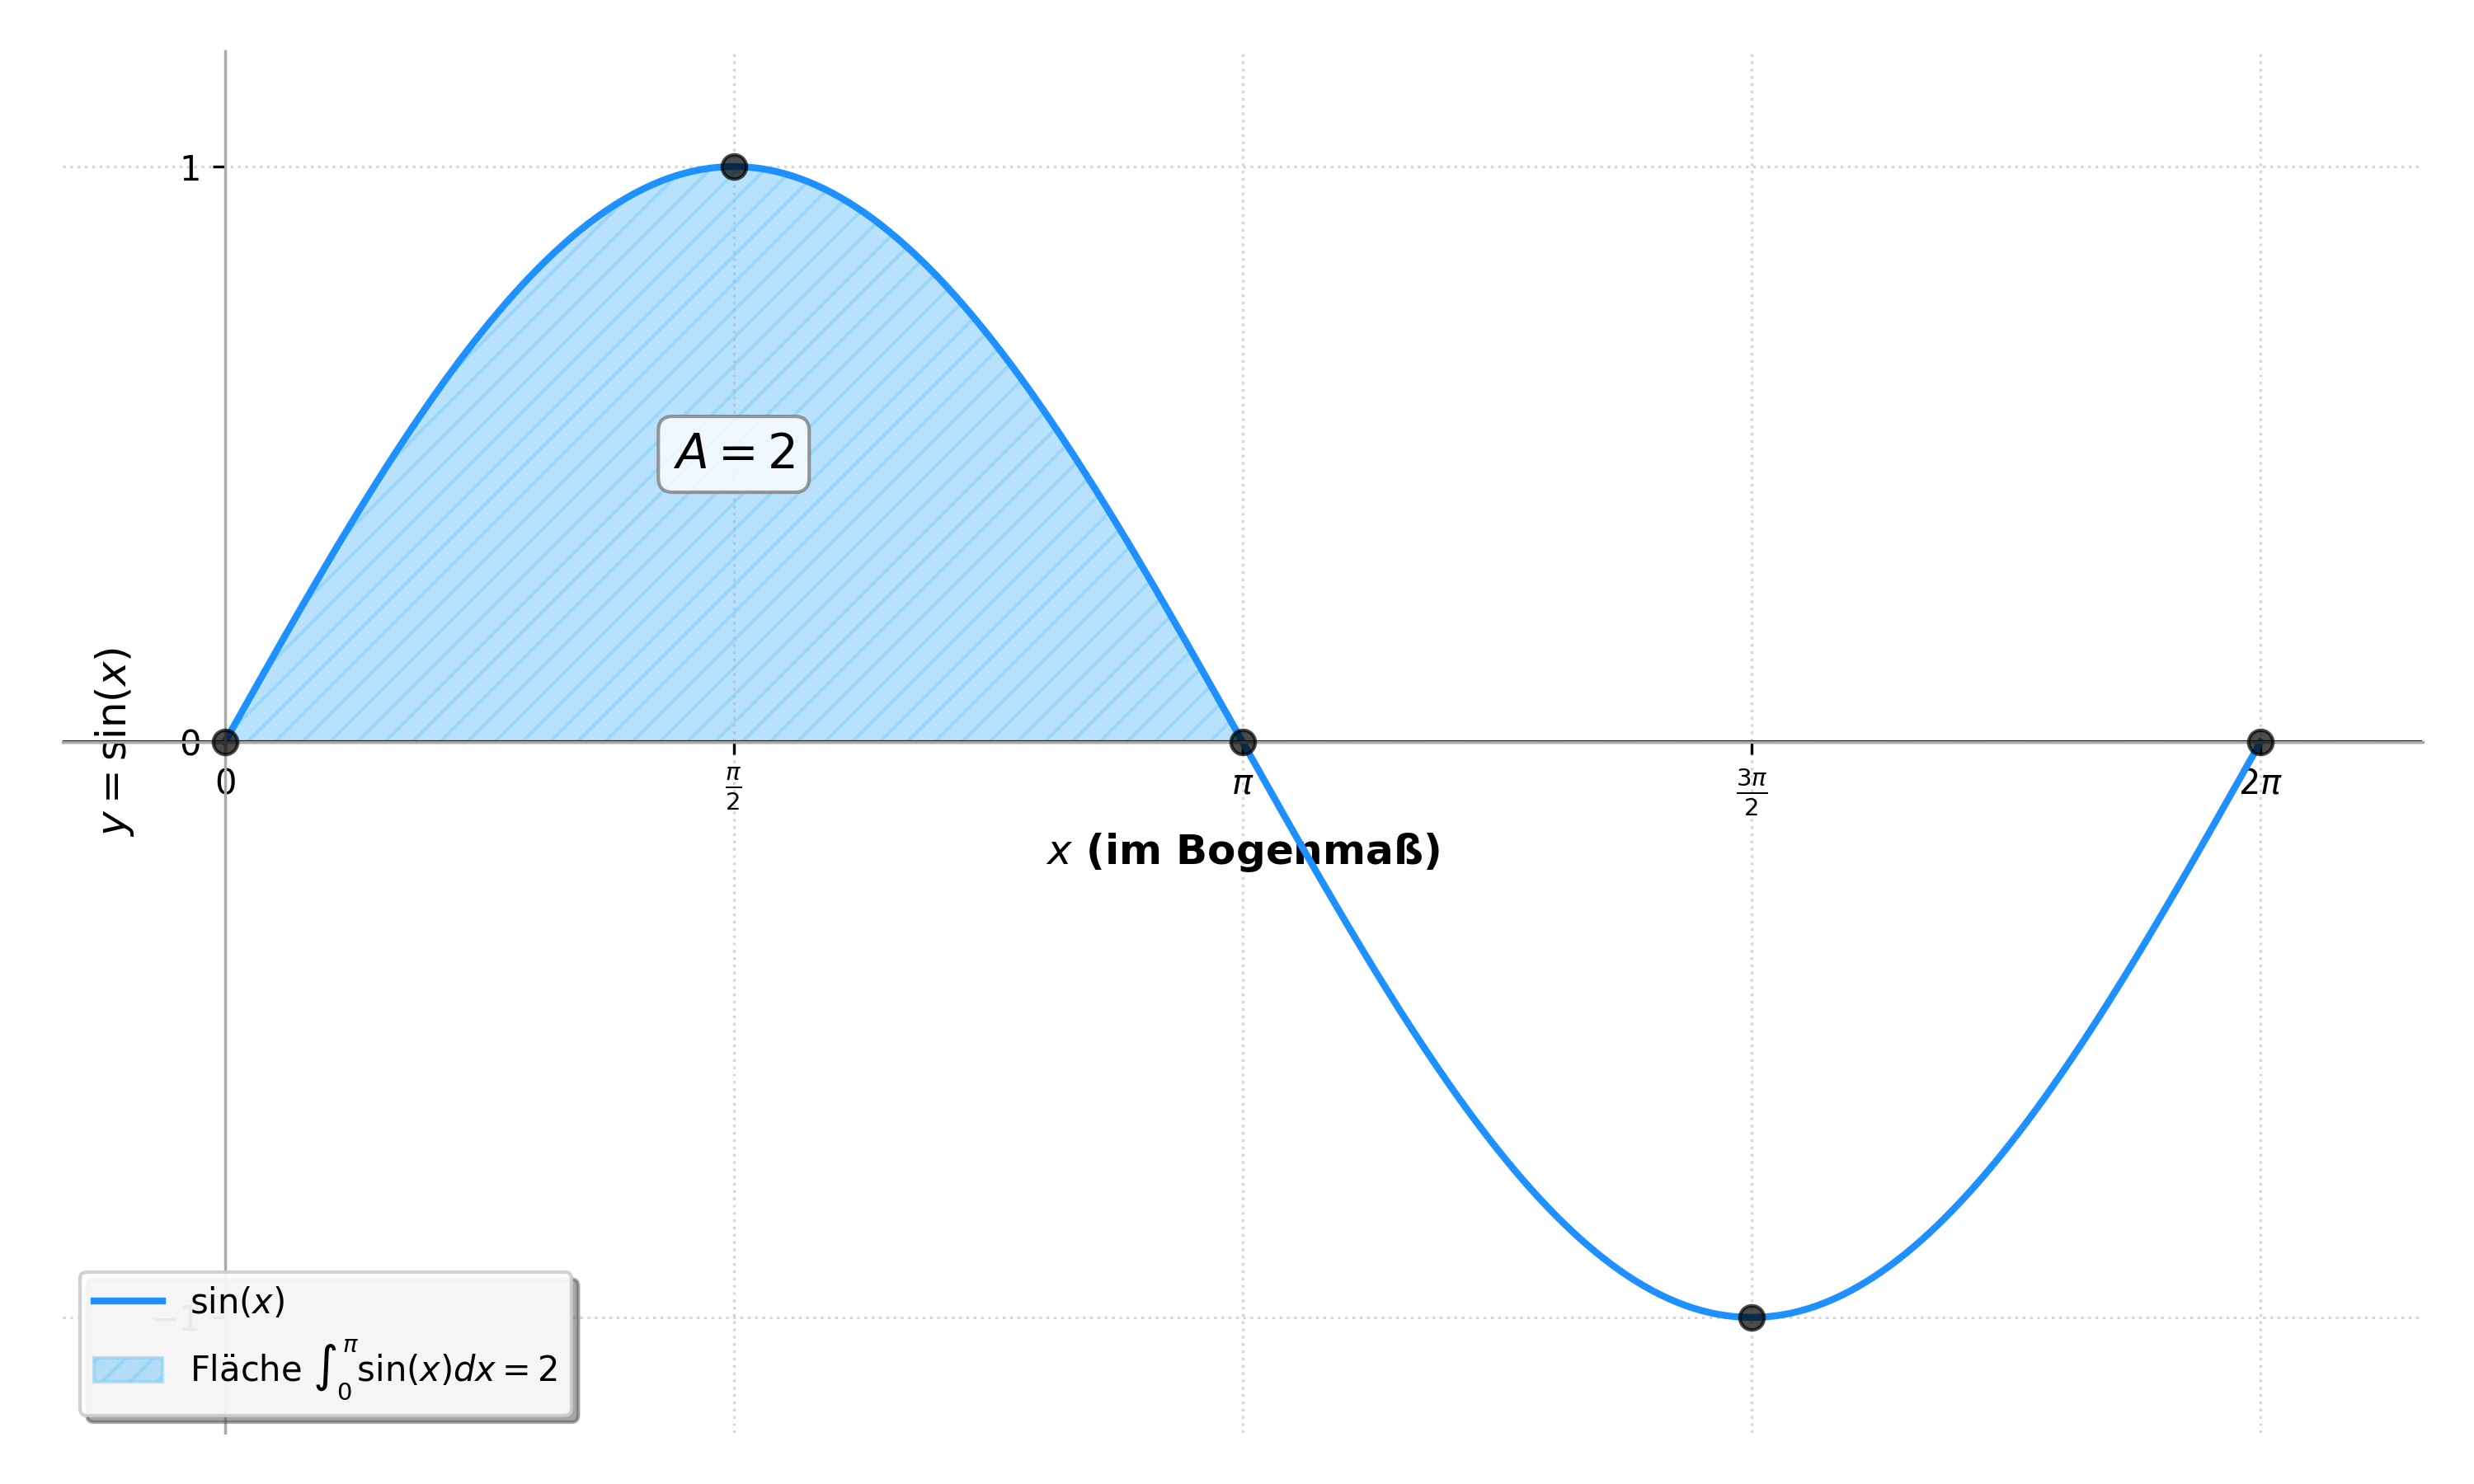
\includegraphics[width=0.8\textwidth]{grafiken/sinus_flaeche_0_pi.png}
    % --- Beschreibung der Skizze ---
    % Die Skizze zeigt den Graphen der Sinusfunktion y = sin(x) für x von 0 bis 2*pi.
    % Die x-Achse ist markiert mit 0, pi/2, pi, 3pi/2, 2pi.
    % Die y-Achse ist markiert mit -1, 0, 1.
    % Der 'erste Berg' der Sinuskurve im Intervall [0, pi] ist schraffiert oder farblich hervorgehoben.
    % Diese Fläche hat den Inhalt 2.
    \captionof{figure}{Graph von $\sin(x)$ mit markierter Fläche $\int_0^{\pi} \sin(x) \,dx$.}
    \label{fig:sinus_flaeche_0_pi}
    \end{center}

    \item \textbf{Was ist $\int_0^{2\pi} \sin(x) \,dx$? Erkläre das Ergebnis anhand der Symmetrie und der orientierten Fläche.}
    \begin{align*} \int_0^{2\pi} \sin(x) \,dx &= [-\cos(x)]_0^{2\pi} \\ &= (-\cos(2\pi)) - (-\cos(0)) \\ &= (-(1)) - (-1) \\ &= -1 + 1 = \mathbf{0} \end{align*}
    \textbf{Erklärung:}
    Das bestimmte Integral $\int_0^{2\pi} \sin(x) \,dx$ stellt die orientierte Fläche zwischen dem Graphen von $\sin(x)$ und der x-Achse im Intervall $[0, 2\pi]$ dar.
    \begin{itemize}
        \item Im Intervall $[0, \pi]$ verläuft der Graph von $\sin(x)$ oberhalb der x-Achse. Der Flächeninhalt dieses Teils ist, wie in c) berechnet, $+2$.
        \item Im Intervall $[\pi, 2\pi]$ verläuft der Graph von $\sin(x)$ unterhalb der x-Achse. Aufgrund der Symmetrie der Sinusfunktion (punktsymmetrisch zu $(\pi|0)$ oder durch Verschiebung des ersten 'Berges') ist der Flächeninhalt dieses Teils dem Betrag nach ebenfalls $2$, aber da er unterhalb der x-Achse liegt, geht er mit negativem Vorzeichen in das bestimmte Integral ein: $\int_{\pi}^{2\pi} \sin(x) \,dx = -2$.
    \end{itemize}
    Die Gesamtbilanz der orientierten Flächen ist somit $\int_0^{2\pi} \sin(x) \,dx = \int_0^{\pi} \sin(x) \,dx + \int_{\pi}^{2\pi} \sin(x) \,dx = 2 + (-2) = 0$.
    Die positive Fläche im ersten Teil des Intervalls und die negative Fläche im zweiten Teil heben sich exakt auf.
\end{enumerate}

\end{loesungsumgebung}



\begin{aufgabenumgebung}{Transformierte Sinus- und Kosinusfunktionen}
\begin{enumerate}
    \item Bestimme für die folgenden Funktionen Amplitude, Periode, Phasenverschiebung (Richtung und Betrag) und Verschiebung in y-Richtung. Gib den Wertebereich an.
        \begin{itemize}
            \item $f_1(x) = 3 \cos(2x - \pi) - 1$ (Tipp: Klammere zuerst den Faktor vor dem $x$ in der Klammer aus, um die Form $B(x-C)$ zu erhalten: $2x-\pi = 2(x-\frac{\pi}{2})$)
            \item $f_2(x) = -0.5 \sin(\pi x + \frac{\pi}{4}) + 2$
            \item $f_3(t) = 100 \cos(2\pi \cdot 50 t)$ (Modell für Wechselspannung)
        \end{itemize}
    \item Skizziere den Graphen von $g(x) = \sin(2(x+\frac{\pi}{4}))$ für eine Periode. Beginne mit dem Graphen von $\sin(x)$ und führe die Transformationen schrittweise durch.
    \item Gegeben ist ein Graph einer Sinusfunktion. Bestimme aus dem Graphen die Parameter $A, B, C, D$ und stelle eine mögliche Funktionsgleichung auf.
        \begin{center}
            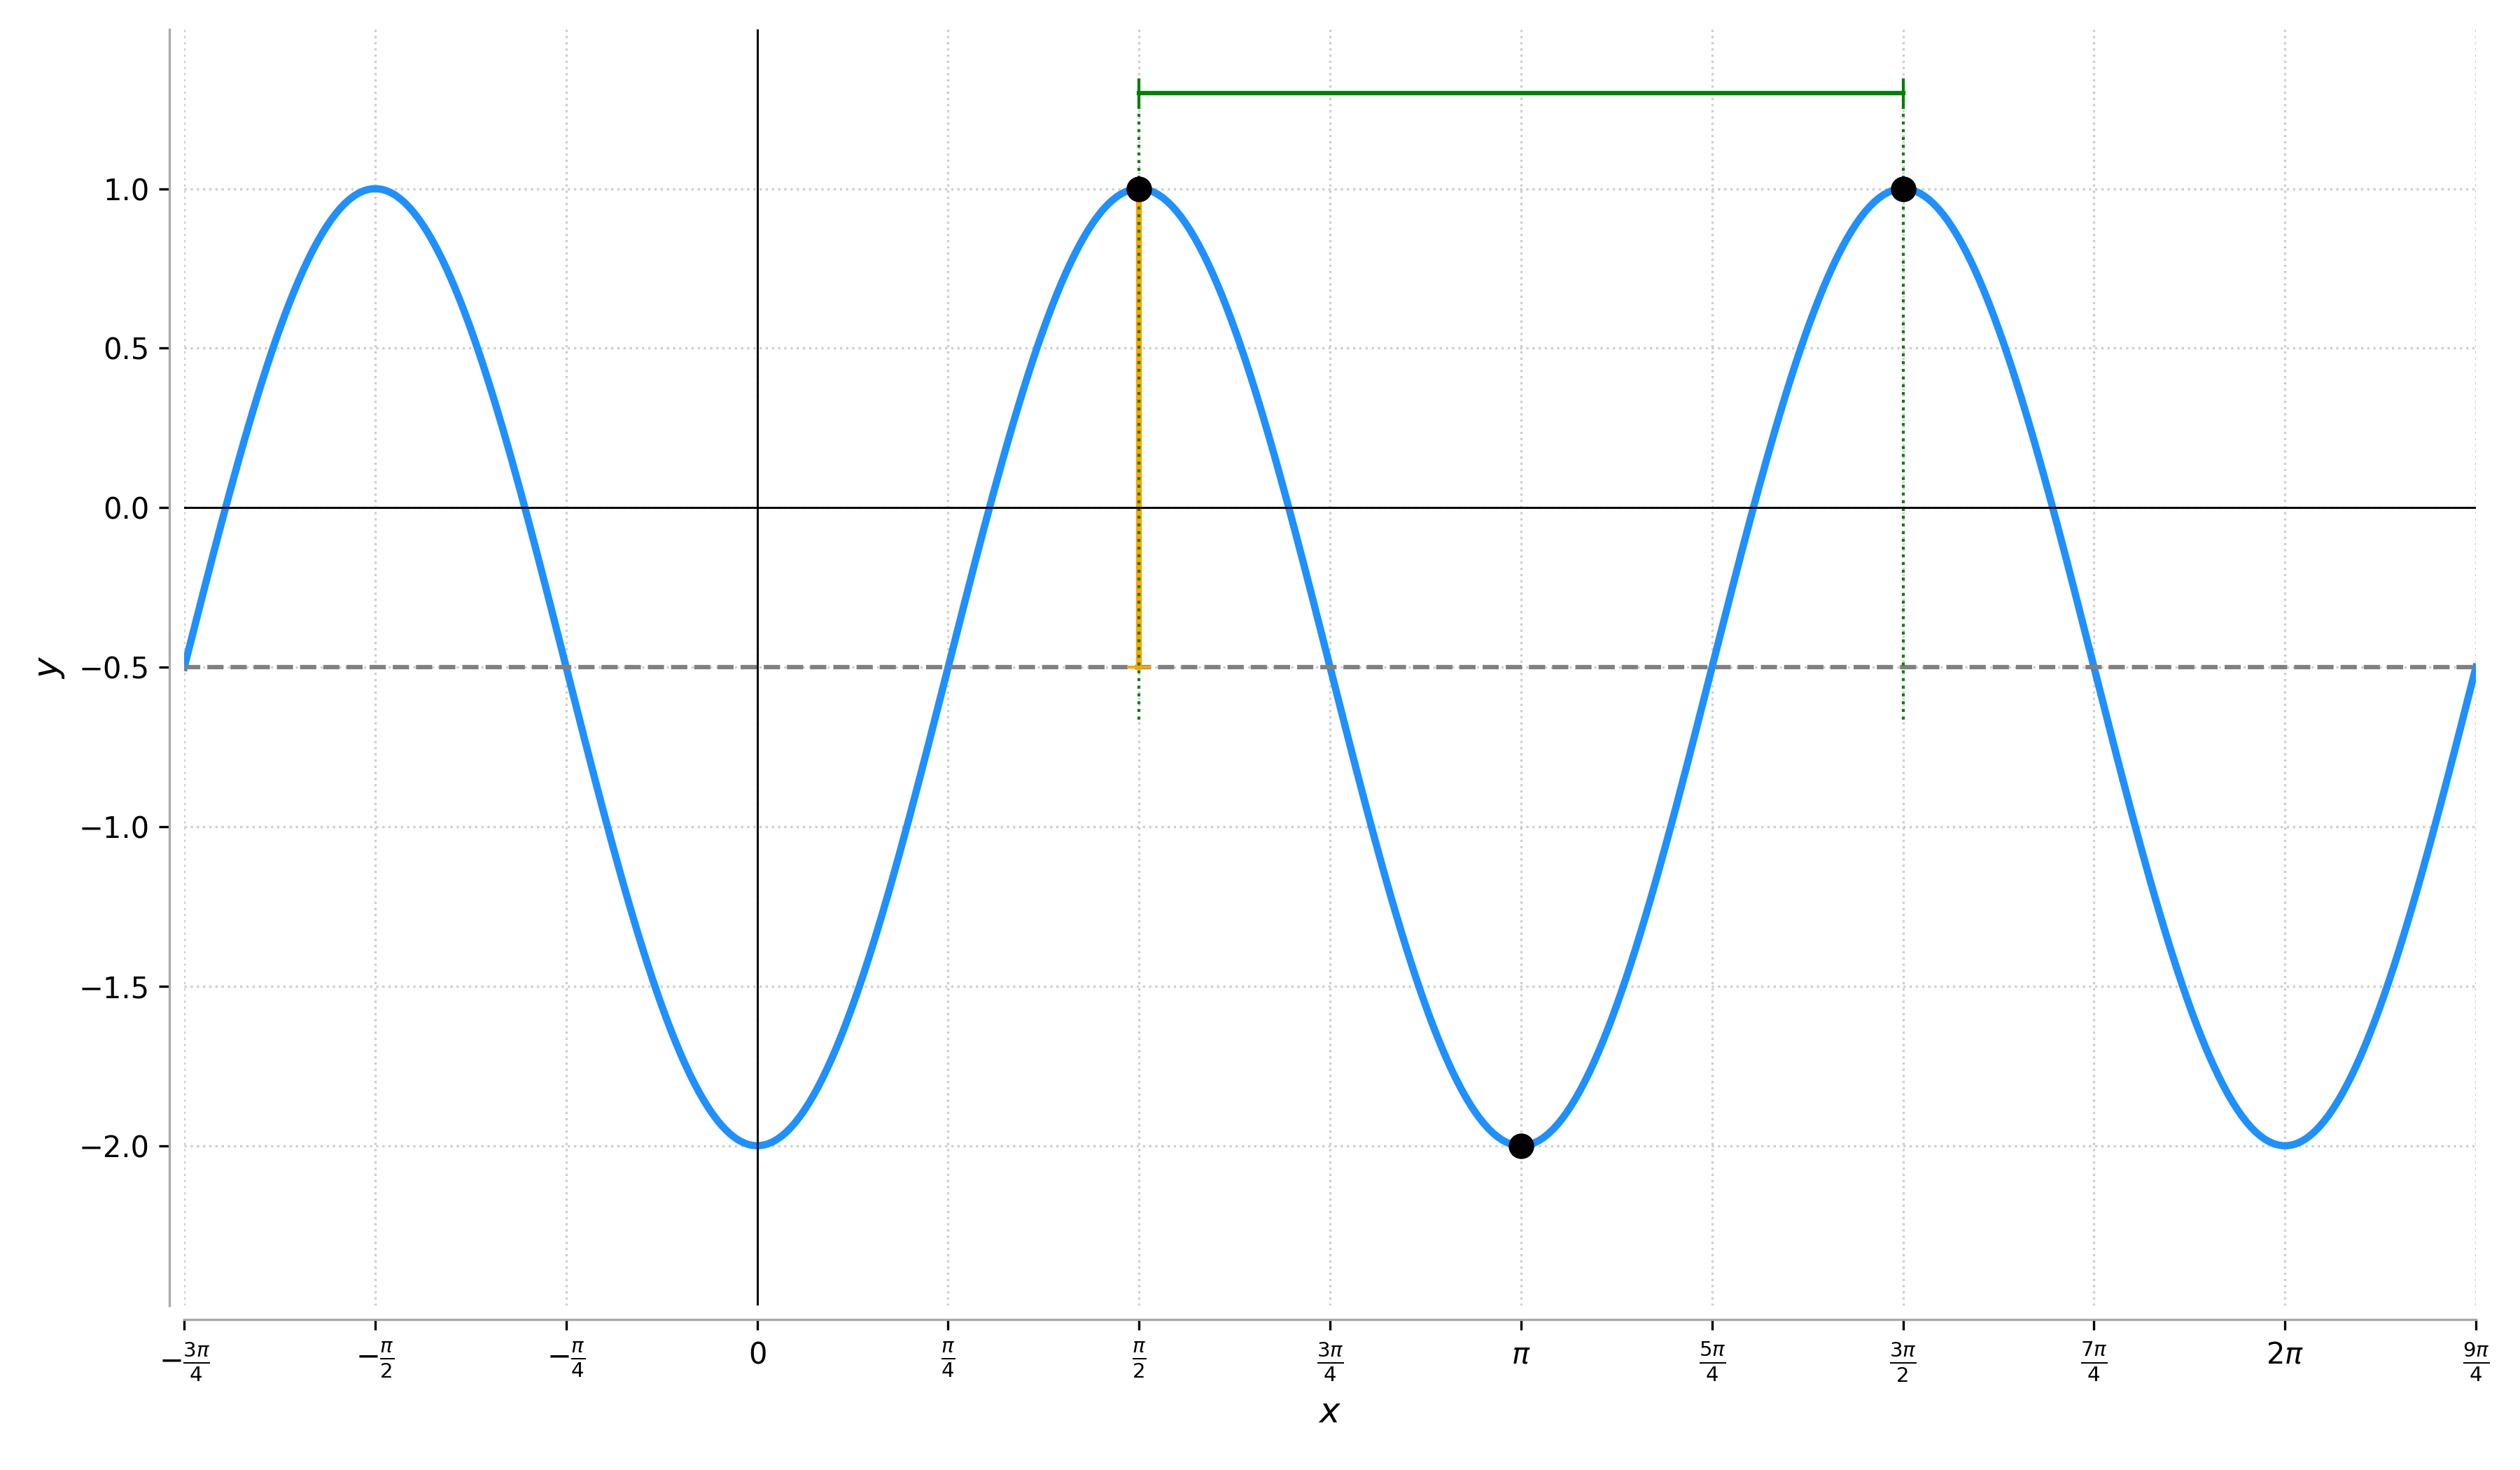
\includegraphics[width=0.7\textwidth]{grafiken/Trig_Graph_Ablesen(1).png}
            \captionof{figure}{Graph zum Ablesen der Parameter}
            \label{fig:graph_ablesen}
        \end{center}
\end{enumerate}
\end{aufgabenumgebung}

\begin{loesungsumgebung}[loes:transformierte-sin-cos-funktionen]{Transformierte Sinus- und Kosinusfunktionen}

\begin{enumerate}[label=(\alph*)]
    \item \textbf{Bestimmung von Amplitude, Periode, Phasenverschiebung, y-Verschiebung und Wertebereich:}
    \begin{itemize}
        \item \textbf{$f_1(x) = 3 \cos(2x - \pi) - 1$} \\
        Umformung des Arguments: $2x - \pi = 2(x - \frac{\pi}{2})$.
        Also $f_1(x) = 3 \cos\left(2\left(x - \frac{\pi}{2}\right)\right) - 1$.
        Hier ist $A=3$, $B=2$, $C=\frac{\pi}{2}$, $D=-1$.
        \begin{itemize}
            \item \textbf{Amplitude:} $|A| = |3| = 3$.
            \item \textbf{Periode:} $P = \frac{2\pi}{|B|} = \frac{2\pi}{2} = \pi$.
            \item \textbf{Phasenverschiebung:} $C = \frac{\pi}{2}$ nach rechts.
            \item \textbf{Verschiebung in y-Richtung:} $D = -1$ (Mittellinie $y=-1$).
            \item \textbf{Wertebereich:} $[D-|A|, D+|A|] = [-1-3, -1+3] = \mathbf{[-4, 2]}$.
        \end{itemize}

        \item \textbf{$f_2(x) = -0.5 \sin(\pi x + \frac{\pi}{4}) + 2$} \\
        Umformung des Arguments: $\pi x + \frac{\pi}{4} = \pi(x + \frac{1}{4}) = \pi(x - (-\frac{1}{4}))$.
        Also $f_2(x) = -0.5 \sin\left(\pi\left(x - \left(-\frac{1}{4}\right)\right)\right) + 2$.
        Hier ist $A=-0.5$, $B=\pi$, $C=-\frac{1}{4}$, $D=2$.
        \begin{itemize}
            \item \textbf{Amplitude:} $|A| = |-0.5| = 0.5$. (Das negative Vorzeichen bei $A$ bedeutet eine Spiegelung an der Mittellinie).
            \item \textbf{Periode:} $P = \frac{2\pi}{|B|} = \frac{2\pi}{\pi} = 2$.
            \item \textbf{Phasenverschiebung:} $C = -\frac{1}{4}$ (d.h. um $\frac{1}{4}$ nach links).
            \item \textbf{Verschiebung in y-Richtung:} $D = 2$ (Mittellinie $y=2$).
            \item \textbf{Wertebereich:} $[D-|A|, D+|A|] = [2-0.5, 2+0.5] = \mathbf{[1.5, 2.5]}$.
        \end{itemize}

        \item \textbf{$f_3(t) = 100 \cos(2\pi \cdot 50 t)$} \\
        Dies kann geschrieben werden als $f_3(t) = 100 \cos(100\pi t)$.
        Hier ist $A=100$, $B=100\pi$, $C=0$, $D=0$.
        \begin{itemize}
            \item \textbf{Amplitude:} $|A| = |100| = 100$.
            \item \textbf{Periode:} $P = \frac{2\pi}{|B|} = \frac{2\pi}{100\pi} = \frac{1}{50}$.
            \item \textbf{Phasenverschiebung:} $C = 0$.
            \item \textbf{Verschiebung in y-Richtung:} $D = 0$ (Mittellinie $y=0$).
            \item \textbf{Wertebereich:} $[D-|A|, D+|A|] = [0-100, 0+100] = \mathbf{[-100, 100]}$.
        \end{itemize}
    \end{itemize}

    \item \textbf{Skizziere den Graphen von $g(x) = \sin(2(x+\frac{\pi}{4}))$ für eine Periode (textuelle Beschreibung).}
    Die Funktion ist $g(x) = \sin(2(x - (-\frac{\pi}{4})))$.
    Parameter: Amplitude $A=1$, $B=2$, Phasenverschiebung $C=-\frac{\pi}{4}$ (nach links), y-Verschiebung $D=0$.
    Periode $P = \frac{2\pi}{2} = \pi$.
    \textbf{Transformationsschritte von $\sin(x)$ zu $g(x)$:}
    \begin{enumerate}
        \item \textit{Grundfunktion $y_0 = \sin(x)$:} Periode $2\pi$, Nullstellen bei $k\pi$, Wertebereich $[-1,1]$.
        \item \textit{Horizontale Stauchung ($B=2$): $y_1 = \sin(2x)$.} Die Periode wird halbiert zu $P=\pi$. Nullstellen bei $k\frac{\pi}{2}$.
        \item \textit{Phasenverschiebung ($C=-\frac{\pi}{4}$): $g(x) = \sin(2(x+\frac{\pi}{4}))$.} Der Graph von $\sin(2x)$ wird um $\frac{\pi}{4}$ nach links verschoben.
    \end{enumerate}
    \textbf{Charakteristische Punkte für eine Periode von $g(x)$:}
    Der 'Start' einer Sinusperiode (Argument ist $0$) liegt bei $2(x+\frac{\pi}{4})=0 \Rightarrow x+\frac{\pi}{4}=0 \Rightarrow x=-\frac{\pi}{4}$.
    \begin{itemize}
        \item Startpunkt (Nullstelle, steigend): $(-\frac{\pi}{4}, 0)$.
        \item Hochpunkt: Eine Viertelperiode weiter rechts: $x = -\frac{\pi}{4} + \frac{P}{4} = -\frac{\pi}{4} + \frac{\pi}{4} = 0$. $g(0) = \sin(2(0+\frac{\pi}{4})) = \sin(\frac{\pi}{2}) = 1$. Punkt $(0,1)$.
        \item Nächste Nullstelle (fallend): Eine halbe Periode vom Start: $x = -\frac{\pi}{4} + \frac{P}{2} = -\frac{\pi}{4} + \frac{\pi}{2} = \frac{\pi}{4}$. $g(\frac{\pi}{4}) = \sin(2(\frac{\pi}{4}+\frac{\pi}{4})) = \sin(\pi) = 0$. Punkt $(\frac{\pi}{4},0)$.
        \item Tiefpunkt: Dreiviertel einer Periode vom Start: $x = -\frac{\pi}{4} + \frac{3P}{4} = -\frac{\pi}{4} + \frac{3\pi}{4} = \frac{2\pi}{4} = \frac{\pi}{2}$. $g(\frac{\pi}{2}) = \sin(2(\frac{\pi}{2}+\frac{\pi}{4})) = \sin(2 \cdot \frac{3\pi}{4}) = \sin(\frac{3\pi}{2}) = -1$. Punkt $(\frac{\pi}{2},-1)$.
        \item Endpunkt einer Periode (Nullstelle, steigend): Eine volle Periode vom Start: $x = -\frac{\pi}{4} + P = -\frac{\pi}{4} + \pi = \frac{3\pi}{4}$. $g(\frac{3\pi}{4})=0$. Punkt $(\frac{3\pi}{4},0)$.
    \end{itemize}
    Eine Periode verläuft also z.B. im Intervall $[-\frac{\pi}{4}, \frac{3\pi}{4}]$. Der Graph steigt von $(-\frac{\pi}{4},0)$ zum Hochpunkt $(0,1)$, fällt durch $(\frac{\pi}{4},0)$ zum Tiefpunkt $(\frac{\pi}{2},-1)$ und steigt wieder zu $(\frac{3\pi}{4},0)$.

    \item \textbf{Parameter aus dem Graphen (Abbildung \ref{fig:graph_ablesen} bzw. die hochgeladene Abbildung) bestimmen:}
    \begin{itemize}
        \item \textbf{Mittellinie $D$:} Der Graph schwankt zwischen $y_{max}=1$ und $y_{min}=-2$.
        $D = \frac{y_{max} + y_{min}}{2} = \frac{1 + (-2)}{2} = \frac{-1}{2} = \mathbf{-0.5}$.
        \item \textbf{Amplitude $|A|$:} $|A| = \frac{y_{max} - y_{min}}{2} = \frac{1 - (-2)}{2} = \frac{3}{2} = \mathbf{1.5}$.
        \item \textbf{Periode $P$:} Ein Hochpunkt ist bei $x \approx \pi/2$. Der nächste Hochpunkt (aus der Symmetrie der Sinus-/Kosinusform erschlossen, im Bild bei $5\pi/2$ klar erkennbar) ist bei $x \approx \pi/2 + P$. Der Abstand zwischen den Hochpunkten bei $x=\pi/2$ und $x=5\pi/2$ ist $P = \frac{5\pi}{2} - \frac{\pi}{2} = \frac{4\pi}{2} = \mathbf{2\pi}$.
        \item \textbf{Parameter $B$:} $P = \frac{2\pi}{|B|} \Rightarrow 2\pi = \frac{2\pi}{|B|} \Rightarrow |B|=1$. Wir wählen $\mathbf{B=1}$ (Standardorientierung).
        \item \textbf{Phasenverschiebung $C$ und Wahl von $A$ (Sinusform $f(x) = A \sin(B(x-C)) + D$):}
        Wir haben $D=-0.5$ und $|A|=1.5$.
        Der Graph schneidet die Mittellinie $y=-0.5$ bei $x=0$ mit positivem Anstieg. Dies kann als Startpunkt einer nicht-gespiegelten Sinusfunktion ($A=1.5$) betrachtet werden.
        Wenn dies der Startpunkt ist, ist die Phasenverschiebung $C=0$.
        Mögliche Funktionsgleichung: $f(x) = 1.5 \sin(1(x-0)) - 0.5 = \mathbf{1.5 \sin(x) - 0.5}$.
        \textit{Überprüfung mit markanten Punkten aus dem typischen Bild:}
        \begin{itemize}
            \item $f(0) = 1.5 \sin(0) - 0.5 = -0.5$. (Passt zum Schnitt mit y-Achse auf Mittellinie).
            \item $f(\pi/2) = 1.5 \sin(\pi/2) - 0.5 = 1.5(1) - 0.5 = 1$. (Passt zum Hochpunkt).
            \item $f(\pi) = 1.5 \sin(\pi) - 0.5 = 1.5(0) - 0.5 = -0.5$. (Schnitt mit Mittellinie).
            \item $f(3\pi/2) = 1.5 \sin(3\pi/2) - 0.5 = 1.5(-1) - 0.5 = -1.5 - 0.5 = -2$. (Passt zum Tiefpunkt).
        \end{itemize}
        Die Parameter sind also: $\mathbf{A=1.5}$, $\mathbf{B=1}$, $\mathbf{C=0}$, $\mathbf{D=-0.5}$.
        Die Funktionsgleichung ist $f(x) = 1.5 \sin(x) - 0.5$.
    \end{itemize}
\end{enumerate}

\end{loesungsumgebung}





\begin{aufgabenumgebung}{Ableiten mit Tangens}
Bilde die erste Ableitung der folgenden Funktionen:
\begin{enumerate}
    \item $f(x) = 3\tan(x) - x$
    \item $g(x) = x \cdot \tan(x)$ (Produktregel!)
    \item $h(x) = \tan(2x+1)$ (Kettenregel! Äußere Funktion $\tan(u)$, innere $u=2x+1$)
\end{enumerate}
\end{aufgabenumgebung}

\begin{loesungsumgebung}[loes:ableiten-mit-tangens]{Ableiten mit Tangens}
Wir verwenden die Ableitungsregel $(\tan x)' = \frac{1}{\cos^2 x}$ (oder $1+\tan^2 x$) sowie die Summen-, Faktor-, Produkt- und Kettenregel.

\begin{enumerate}[label=(\alph*)]
    \item \textbf{Funktion $f(x) = 3\tan(x) - x$} \\
    Wir leiten die Terme einzeln ab:
    \begin{itemize}
        \item $(3\tan(x))' = 3 \cdot (\tan(x))' = 3 \cdot \frac{1}{\cos^2(x)} = \frac{3}{\cos^2(x)}$.
        \item $(-x)' = -1$.
    \end{itemize}
    Somit ist die Ableitung:
    $$ f'(x) = \mathbf{\frac{3}{\cos^2(x)} - 1} $$
    Alternativ, mit $(\tan x)' = 1+\tan^2 x$:
    $f'(x) = 3(1+\tan^2 x) - 1 = 3+3\tan^2 x - 1 = \mathbf{2+3\tan^2 x}$.

    \item \textbf{Funktion $g(x) = x \cdot \tan(x)$} (Produktregel!) \\
    Wir wenden die Produktregel $(uv)' = u'v + uv'$ an.
    Sei $u(x) = x \Rightarrow u'(x) = 1$. \\
    Sei $v(x) = \tan(x) \Rightarrow v'(x) = \frac{1}{\cos^2(x)}$.
    \begin{align*}
    g'(x) &= u'(x)v(x) + u(x)v'(x) \\
            &= 1 \cdot \tan(x) + x \cdot \frac{1}{\cos^2(x)} \\
            &= \mathbf{\tan(x) + \frac{x}{\cos^2(x)}}
    \end{align*}
    Alternativ, mit $v'(x) = 1+\tan^2 x$:
    $g'(x) = \tan(x) + x(1+\tan^2 x) = \tan(x) + x + x\tan^2 x$.

    \item \textbf{Funktion $h(x) = \tan(2x+1)$} (Kettenregel!) \\
    Wir wenden die Kettenregel $(a(i(x)))' = a'(i(x)) \cdot i'(x)$ an.
    \begin{itemize}
        \item Äußere Funktion: $a(u) = \tan(u) \Rightarrow a'(u) = \frac{1}{\cos^2(u)}$.
        \item Innere Funktion: $i(x) = 2x+1 \Rightarrow i'(x) = 2$.
    \end{itemize}
    Anwendung der Kettenregel:
    \begin{align*}
    h'(x) &= a'(i(x)) \cdot i'(x) \\
            &= \frac{1}{\cos^2(2x+1)} \cdot 2 \\
            &= \mathbf{\frac{2}{\cos^2(2x+1)}}
    \end{align*}
    Alternativ, mit $a'(u) = 1+\tan^2 u$:
    $h'(x) = (1+\tan^2(2x+1)) \cdot 2 = \mathbf{2(1+\tan^2(2x+1))}$.
\end{enumerate}

\end{loesungsumgebung}





\begin{aufgabenumgebung}{Ableiten trigonometrischer Funktionskombinationen}
Bilde die erste Ableitung der folgenden Funktionen und vereinfache, wenn möglich.
\begin{enumerate}
    \item $f_1(x) = (x^3+1)\cos(x)$
    \item $f_2(x) = \frac{\sin(x)}{e^x}$
    \item $f_3(x) = \cos(x^2+1)$
    \item $f_4(x) = \sin^2(x)$ (Tipp: $\sin^2(x) = (\sin x)^2$. Kettenregel!)
    \item $f_5(x) = \ln(\cos x)$ (Für welche $x$ ist dies definiert?)
    \item $f_6(x) = e^{\sin(x)}$
\end{enumerate}
\end{aufgabenumgebung}

\begin{loesungsumgebung}[loes:ableiten-trig-kombinationen]{Ableiten trigonometrischer Funktionskombinationen}
Wir bilden die erste Ableitung der gegebenen Funktionen und vereinfachen die Ergebnisse, wo möglich.

\begin{enumerate}[label=(\alph*)]
    \item \textbf{Funktion $f_1(x) = (x^3+1)\cos(x)$} \\
    Anwendung der Produktregel: $u(x) = x^3+1 \Rightarrow u'(x) = 3x^2$. $v(x) = \cos(x) \Rightarrow v'(x) = -\sin(x)$.
    \begin{align*}
    f_1'(x) &= u'(x)v(x) + u(x)v'(x) \\
            &= (3x^2)(\cos(x)) + (x^3+1)(-\sin(x)) \\
            &= \mathbf{3x^2\cos(x) - (x^3+1)\sin(x)}
    \end{align*}

    \item \textbf{Funktion $f_2(x) = \frac{\sin(x)}{e^x}$} \\
    Anwendung der Quotientenregel: $u(x) = \sin(x) \Rightarrow u'(x) = \cos(x)$. $v(x) = e^x \Rightarrow v'(x) = e^x$.
    \begin{align*}
    f_2'(x) &= \frac{u'(x)v(x) - u(x)v'(x)}{[v(x)]^2} \\
            &= \frac{\cos(x)e^x - \sin(x)e^x}{(e^x)^2} \\
            &= \frac{e^x(\cos(x) - \sin(x))}{e^{2x}} \\
            &= \mathbf{\frac{\cos(x) - \sin(x)}{e^x}} \quad \text{oder} \quad \mathbf{(\cos(x) - \sin(x))e^{-x}}
    \end{align*}

    \item \textbf{Funktion $f_3(x) = \cos(x^2+1)$} \\
    Anwendung der Kettenregel: Äußere Funktion $a(u) = \cos(u) \Rightarrow a'(u) = -\sin(u)$. Innere Funktion $i(x) = x^2+1 \Rightarrow i'(x) = 2x$.
    \begin{align*}
    f_3'(x) &= a'(i(x)) \cdot i'(x) \\
            &= -\sin(x^2+1) \cdot (2x) \\
            &= \mathbf{-2x\sin(x^2+1)}
    \end{align*}

    \item \textbf{Funktion $f_4(x) = \sin^2(x)$} \\
    Wir schreiben $f_4(x) = (\sin x)^2$ und wenden die Kettenregel an.
    Äußere Funktion $a(u) = u^2 \Rightarrow a'(u) = 2u$. Innere Funktion $i(x) = \sin x \Rightarrow i'(x) = \cos x$.
    \begin{align*}
    f_4'(x) &= a'(i(x)) \cdot i'(x) \\
            &= 2(\sin x) \cdot \cos x \\
            &= \mathbf{2\sin x \cos x}
    \end{align*}
    (Dies ist auch gleich $\sin(2x)$ nach den Doppelwinkelfunktionen).

    \item \textbf{Funktion $f_5(x) = \ln(\cos x)$} \\
    \textbf{Definitionsbereich:} Damit $\ln(\cos x)$ definiert ist, muss $\cos x > 0$ sein. Dies ist z.B. der Fall für $x \in (-\frac{\pi}{2} + 2k\pi, \frac{\pi}{2} + 2k\pi)$ für $k \in \mathbb{Z}$.
    Anwendung der Kettenregel: Äußere Funktion $a(u) = \ln u \Rightarrow a'(u) = \frac{1}{u}$. Innere Funktion $i(x) = \cos x \Rightarrow i'(x) = -\sin x$.
    \begin{align*}
    f_5'(x) &= a'(i(x)) \cdot i'(x) \\
            &= \frac{1}{\cos x} \cdot (-\sin x) \\
            &= -\frac{\sin x}{\cos x} \\
            &= \mathbf{-\tan x}
    \end{align*}
    Die Ableitung ist definiert, wo $\cos x \neq 0$ ist (was bereits durch den Definitionsbereich von $\ln(\cos x)$ sichergestellt ist, da $\cos x > 0$ sein muss).

    \item \textbf{Funktion $f_6(x) = e^{\sin(x)}$} \\
    Anwendung der Kettenregel: Äußere Funktion $a(u) = e^u \Rightarrow a'(u) = e^u$. Innere Funktion $i(x) = \sin x \Rightarrow i'(x) = \cos x$.
    \begin{align*}
    f_6'(x) &= a'(i(x)) \cdot i'(x) \\
            &= e^{\sin x} \cdot \cos x \\
            &= \mathbf{\cos x \cdot e^{\sin x}}
    \end{align*}
\end{enumerate}

\end{loesungsumgebung}




\begin{aufgabenumgebung}{Kurvendiskussionen mit trigonometrischen Funktionen – Analyse und digitale Helfer}
Führe eine möglichst vollständige Kurvendiskussion für die folgenden Funktionen im angegebenen Intervall durch und skizziere den Graphen. Bestimme alle Eigenschaften (Definitionsbereich, Symmetrie, Verhalten an den Rändern, y-Achsenabschnitt, Ableitungen, Monotonie, Krümmung) analytisch, soweit dies mit den dir bekannten Methoden möglich ist. 

Für Nullstellen oder die x-Koordinaten von Extrem- und Wendepunkten, deren exakte Berechnung auf \textbf{transzendente Gleichungen} führt (Gleichungen, die algebraisch nicht einfach nach der Variablen aufgelöst werden können, z.B. wenn $x$ sowohl innerhalb als auch außerhalb einer trigonometrischen Funktion steht), ist eine exakte algebraische Lösung oft nicht das Ziel.
\begin{itemize}
    \item Versuche in solchen Fällen, die \textit{Existenz} von Lösungen durch Überlegungen (z.B. Zwischenwertsatz, falls bekannt, oder Monotonie) zu begründen oder zumindest plausibel zu machen.
    \item Du kannst dann \textbf{digitale Werkzeuge} (wie Wolfram Alpha, GeoGebra oder einen grafikfähigen Taschenrechner) verwenden, um Näherungswerte für diese speziellen x-Werte zu ermitteln. Notiere in deiner Lösung, wenn du solche Näherungswerte verwendest, um deine Skizze zu vervollständigen und die Analyse abzurunden.
\end{itemize}
Der Schwerpunkt liegt auf dem Verständnis der analytischen Schritte und der Interpretation der Ergebnisse.

\begin{enumerate}
    \item $f(x) = 2\sin(x) - x$ im Intervall $[0, 2\pi]$.
        \begin{tippumgebung}{Umgang mit Nullstellen von $f(x)$}
        Du wirst feststellen, dass $x=0$ eine Nullstelle ist. Die Gleichung $2\sin(x) = x$ für weitere Nullstellen ist transzendent. Du kannst grafisch argumentieren, dass es eine weitere Nullstelle im Intervall gibt (z.B. indem du $y=2\sin x$ und $y=x$ vergleichst) oder deren ungefähre Lage mit einem digitalen Werkzeug bestimmen. Konzentriere dich ansonsten auf die exakte Berechnung der Ableitungen, Extrem- und Wendestellen, soweit möglich.
        \end{tippumgebung}
    \item $g(x) = x \cdot \cos(x)$ im Intervall $[-\pi, \pi]$.
        \begin{tippumgebung}{Umgang mit Extremstellen von $g(x)$}
        Die Nullstellen von $g(x)$ sind exakt bestimmbar. Die notwendige Bedingung für Extremstellen ($g'(x)=0$) führt hier jedoch auf die transzendente Gleichung $\cos(x) = x\sin(x)$. Untersuche die Ableitung $g'(x)$ an markanten Punkten (z.B. Nullstellen von $g(x)$ oder Ränder des Intervalls), um Bereiche mit unterschiedlichem Monotonieverhalten zu identifizieren. Für die genaue Lage der Extremstellen kannst du Näherungswerte aus digitalen Werkzeugen verwenden und dies vermerken.
        \end{tippumgebung}
\end{enumerate}
\end{aufgabenumgebung}


\begin{loesungsumgebung}[loes:kurvendiskussion-trig-funktionen]{Kurvendiskussionen mit trigonometrischen Funktionen}
Wir führen für die gegebenen Funktionen eine vollständige Kurvendiskussion im jeweils angegebenen Intervall durch. Die Graphen beider Funktionen sind in der zusammenfassenden Abbildung \ref{fig:kurvendisk_trig_kombiniert} am Ende dieser Lösung konzeptionell dargestellt.

\begin{enumerate}[label=(\alph*)]
    \item \textbf{Funktion $f(x) = 2\sin(x) - x$ im Intervall $[0, 2\pi]$}

    \subsubsection*{1. Definitionsbereich}
    $D_f = [0, 2\pi]$ (laut Aufgabenstellung).

    \subsubsection*{2. Symmetrie}
    $f(-x) = 2\sin(-x) - (-x) = -2\sin x + x$. Da $f(-x) \neq f(x)$ und $f(-x) \neq -f(x)$ (außer für $x=0$), liegt keine einfache Symmetrie zum Ursprung oder zur y-Achse für die allgemeine Funktion vor. Das gegebene Intervall ist zudem nicht symmetrisch zum Ursprung.

    \subsubsection*{3. Verhalten an den Rändern des Definitionsbereichs}
    $f(0) = 2\sin(0) - 0 = 0$.
    $f(2\pi) = 2\sin(2\pi) - 2\pi = 0 - 2\pi = -2\pi \approx -6.283$.

    \subsubsection*{4. Achsenschnittpunkte}
    \begin{itemize}
        \item y-Achsenabschnitt: $P_y(0|0)$ (da $f(0)=0$).
        \item Nullstellen ($f(x)=0$): $2\sin(x) - x = 0 \Rightarrow 2\sin(x) = x$.
        Eine offensichtliche Lösung ist $\mathbf{x_1=0}$.
        Die Aufgabe erwähnt, dass weitere Nullstellen nicht exakt lösbar sind. Eine grafische Betrachtung oder numerische Verfahren würden zeigen, dass es eine weitere Nullstelle im Intervall $(0, 2\pi)$ gibt, etwa bei $x \approx 1.895$. Für die exakte Kurvendiskussion ohne numerische Methoden ist dies aber nicht weiter relevant, wir notieren $x_1=0$.
    \end{itemize}

    \subsubsection*{5. Erste Ableitung $f'(x)$}
    $f'(x) = \frac{d}{dx}(2\sin(x) - x) = \mathbf{2\cos(x) - 1}$.

    \subsubsection*{6. Extrempunkte}
    Notwendige Bedingung: $f'(x_E)=0 \Rightarrow 2\cos(x_E) - 1 = 0 \Rightarrow \cos(x_E) = \frac{1}{2}$.
    Im Intervall $[0, 2\pi]$ sind die Lösungen:
    $x_{E1} = \arccos(\frac{1}{2}) = \frac{\pi}{3}$.
    $x_{E2} = 2\pi - \frac{\pi}{3} = \frac{5\pi}{3}$.
    Zweite Ableitung (siehe unten): $f''(x) = -2\sin(x)$.
    \begin{itemize}
        \item Für $x_{E1} = \frac{\pi}{3}$: $f''(\frac{\pi}{3}) = -2\sin(\frac{\pi}{3}) = -2 \cdot \frac{\sqrt{3}}{2} = -\sqrt{3} < 0 \Rightarrow$ Lokaler Hochpunkt.
        $y_{E1} = f(\frac{\pi}{3}) = 2\sin(\frac{\pi}{3}) - \frac{\pi}{3} = 2\frac{\sqrt{3}}{2} - \frac{\pi}{3} = \sqrt{3} - \frac{\pi}{3} \approx 1.732 - 1.047 \approx 0.685$.
        $\mathbf{HP(\frac{\pi}{3}|\sqrt{3}-\frac{\pi}{3})}$.
        \item Für $x_{E2} = \frac{5\pi}{3}$: $f''(\frac{5\pi}{3}) = -2\sin(\frac{5\pi}{3}) = -2 \cdot (-\frac{\sqrt{3}}{2}) = \sqrt{3} > 0 \Rightarrow$ Lokaler Tiefpunkt.
        $y_{E2} = f(\frac{5\pi}{3}) = 2\sin(\frac{5\pi}{3}) - \frac{5\pi}{3} = 2(-\frac{\sqrt{3}}{2}) - \frac{5\pi}{3} = -\sqrt{3} - \frac{5\pi}{3} \approx -1.732 - 5.236 \approx -6.968$.
        $\mathbf{TP(\frac{5\pi}{3}|-\sqrt{3}-\frac{5\pi}{3})}$.
    \end{itemize}

    \subsubsection*{7. Monotonieverhalten}
    Vorzeichen von $f'(x) = 2\cos(x) - 1$:
    \begin{itemize}
        \item $x \in [0, \frac{\pi}{3})$: $\cos(x) > \frac{1}{2} \Rightarrow f'(x)>0 \Rightarrow f$ streng monoton steigend.
        \item $x \in (\frac{\pi}{3}, \frac{5\pi}{3})$: $\cos(x) < \frac{1}{2} \Rightarrow f'(x)<0 \Rightarrow f$ streng monoton fallend.
        \item $x \in (\frac{5\pi}{3}, 2\pi]$: $\cos(x) > \frac{1}{2} \Rightarrow f'(x)>0 \Rightarrow f$ streng monoton steigend.
    \end{itemize}

    \subsubsection*{8. Zweite Ableitung $f''(x)$}
    $f''(x) = \frac{d}{dx}(2\cos(x) - 1) = \mathbf{-2\sin(x)}$.

    \subsubsection*{9. Wendepunkte}
    Notwendige Bedingung: $f''(x_W)=0 \Rightarrow -2\sin(x_W)=0 \Rightarrow \sin(x_W)=0$.
    Im Intervall $[0, 2\pi]$ sind die Lösungen $x=0, x=\pi, x=2\pi$.
    Wir betrachten $x_W=\pi$ als inneren Punkt. Die Ränder $0$ und $2\pi$ sind keine Wendepunkte im klassischen Sinn.
    Dritte Ableitung: $f'''(x) = -2\cos(x)$.
    $f'''(\pi) = -2\cos(\pi) = -2(-1) = 2 \neq 0$.
    Somit ist bei $x_W=\pi$ ein Wendepunkt.
    $y_W = f(\pi) = 2\sin(\pi) - \pi = 0 - \pi = -\pi$.
    Wendepunkt $\mathbf{W(\pi|-\pi)}$.

    \subsubsection*{10. Krümmungsverhalten}
    Vorzeichen von $f''(x)=-2\sin(x)$:
    \begin{itemize}
        \item $x \in (0, \pi)$: $\sin(x) > 0 \Rightarrow -2\sin(x) < 0 \Rightarrow f''(x) < 0 \Rightarrow f$ ist rechtsgekrümmt.
        \item $x \in (\pi, 2\pi)$: $\sin(x) < 0 \Rightarrow -2\sin(x) > 0 \Rightarrow f''(x) > 0 \Rightarrow f$ ist linksgekrümmt.
    \end{itemize}

    \subsubsection*{11. Wertebereich im Intervall $[0, 2\pi]$}
    $f(0)=0$, $f(2\pi)=-2\pi \approx -6.283$. $HP_y = \sqrt{3}-\pi/3 \approx 0.685$. $TP_y = -\sqrt{3}-5\pi/3 \approx -6.968$.
    Der kleinste Wert ist $y_{TP}$. Der größte Wert ist $y_{HP}$.
    $W_f = [-\sqrt{3}-\frac{5\pi}{3}, \sqrt{3}-\frac{\pi}{3}]$.

    \item \textbf{Funktion $g(x) = x \cdot \cos(x)$ im Intervall $[-\pi, \pi]$}

    \subsubsection*{1. Definitionsbereich}
    $D_g = [-\pi, \pi]$ (laut Aufgabenstellung).

    \subsubsection*{2. Symmetrie}
    $g(-x) = (-x)\cos(-x) = -x\cos(x) = -g(x)$ (da $\cos(-x)=\cos(x)$).
    Die Funktion ist \textbf{punktsymmetrisch zum Ursprung}.

    \subsubsection*{3. Verhalten an den Rändern des Definitionsbereichs}
    $g(-\pi) = -\pi \cos(-\pi) = -\pi(-1) = \pi$.
    $g(\pi) = \pi \cos(\pi) = \pi(-1) = -\pi$.

    \subsubsection*{4. Achsenschnittpunkte}
    \begin{itemize}
        \item y-Achsenabschnitt: $g(0) = 0 \cos(0) = 0$. $P_y(0|0)$.
        \item Nullstellen ($g(x)=0$): $x\cos(x)=0 \Rightarrow x=0$ oder $\cos(x)=0$.
        Im Intervall $[-\pi, \pi]$ gilt $\cos(x)=0$ für $x=-\frac{\pi}{2}$ und $x=\frac{\pi}{2}$.
        Nullstellen: $\mathbf{x_1=-\frac{\pi}{2}, x_2=0, x_3=\frac{\pi}{2}}$.
    \end{itemize}

    \subsubsection*{5. Erste Ableitung $g'(x)$}
    Mit der Produktregel ($u=x, u'=1; v=\cos x, v'=-\sin x$):
    $g'(x) = 1 \cdot \cos(x) + x(-\sin(x)) = \mathbf{\cos(x) - x\sin(x)}$.

    \subsubsection*{6. Extrempunkte}
    Notwendige Bedingung: $g'(x_E)=0 \Rightarrow \cos(x_E) - x_E\sin(x_E) = 0 \Rightarrow \cos(x_E) = x_E\sin(x_E)$.
    Diese transzendente Gleichung ist nicht algebraisch exakt lösbar, außer für $x_E=0$, wo $1=0$ (falsch).
    Numerische Lösungen im Intervall $[-\pi, \pi]$ sind etwa $x_E \approx \pm 0.8603$. Sei $x_{E0} \approx 0.8603$.
    Wegen Punktsymmetrie von $g(x)$ sind die Extrema symmetrisch. Wenn bei $x_{E0}$ ein Max/Min ist, ist bei $-x_{E0}$ ein Min/Max mit $-g(x_{E0})$.
    $g(0.8603) \approx 0.8603 \cos(0.8603) \approx 0.8603 \cdot 0.6523 \approx 0.561$.
    $g(-0.8603) \approx -0.561$.
    Zweite Ableitung (siehe unten): $g''(x) = -2\sin x - x\cos x$.
    $g''(0.8603) \approx -2\sin(0.8603) - 0.8603\cos(0.8603) \approx -2(0.7580) - 0.8603(0.6523) \approx -1.516 - 0.561 = -2.077 < 0$.
    $\implies$ Lokaler Hochpunkt bei $x \approx 0.8603$. $\mathbf{HP(\approx 0.8603 | \approx 0.561)}$.
    $\implies$ Lokaler Tiefpunkt bei $x \approx -0.8603$. $\mathbf{TP(\approx -0.8603 | \approx -0.561)}$.

    \subsubsection*{7. Monotonieverhalten}
    $g'(0)=1$. $g'(\pi/2)=-\pi/2 < 0$. $g'(-\pi/2)=-\pi/2 < 0$. $g'(\pi)=-1$. $g'(-\pi)=-1$.
    $g'(x)$ wechselt Vorzeichen bei $x \approx \pm 0.8603$.
    Fallend in $[-\pi, -0.8603]$, steigend in $[-0.8603, 0.8603]$, fallend in $[0.8603, \pi]$.

    \subsubsection*{8. Zweite Ableitung $g''(x)$}
    $g''(x) = \frac{d}{dx}(\cos x - x\sin x) = -\sin x - (1\cdot\sin x + x\cos x) = \mathbf{-2\sin x - x\cos x}$.

    \subsubsection*{9. Wendepunkte}
    Notwendige Bedingung: $g''(x_W)=0 \Rightarrow -2\sin x_W - x_W\cos x_W = 0$.
    Eine Lösung ist $\mathbf{x_W=0}$. $g(0)=0$.
    $g'''(x) = -2\cos x - (\cos x - x\sin x) = -3\cos x + x\sin x$.
    $g'''(0) = -3\cos 0 + 0 = -3 \neq 0 \implies$ Wendepunkt bei $W_1(0|0)$.
    Weitere Nullstellen von $-2\sin x - x\cos x = 0 \Leftrightarrow 2\tan x = -x$ (für $\cos x \ne 0$) sind numerisch zu finden, etwa $x_{W2} \approx 2.289$ und $x_{W3} \approx -2.289$ (im Intervall $[-\pi,\pi]$ nicht ganz enthalten, $2.289 < \pi \approx 3.14$).
    $x_{W2} \approx 2.289$: $g(2.289) \approx 2.289 \cos(2.289) \approx 2.289(-0.652) \approx -1.492$. $W_2(\approx 2.289 | \approx -1.492)$.
    $x_{W3} \approx -2.289$: $g(-2.289) \approx -2.289 \cos(-2.289) \approx -2.289(-0.652) \approx 1.492$. $W_3(\approx -2.289 | \approx 1.492)$.

    \subsubsection*{10. Krümmungsverhalten}
    Bestimmt durch das Vorzeichen von $g''(x) = -2\sin x - x\cos x$.
    Um $x=0$: $g''(x) \approx -2x - x(1) = -3x$. Wechsel von $+$ nach $-$ bei $x=0$.
    Linksgekrümmt in $(-\pi, \approx -2.289)$ und $(0, \approx 2.289)$.
    Rechtsgekrümmt in $(\approx -2.289, 0)$ und $(\approx 2.289, \pi)$.

    \subsubsection*{11. Wertebereich im Intervall $[-\pi, \pi]$}
    Randwerte: $g(-\pi)=\pi \approx 3.141$, $g(\pi)=-\pi \approx -3.141$.
    Lokale Extrema: $HP_y \approx 0.561$, $TP_y \approx -0.561$.
    Der globale Maximalwert im Intervall ist $\pi$ (bei $x=-\pi$). Der globale Minimalwert ist $-\pi$ (bei $x=\pi$).
    $W_g = [-\pi, \pi]$.
\end{enumerate}

\subsubsection*{Gemeinsame Skizze der Graphen}
Eine Darstellung beider Graphen in einem Koordinatensystem.
\begin{itemize}
    \item $f(x)=2\sin x - x$: Startet bei $(0|0)$, hat HP bei $(\pi/3|\sqrt{3}-\pi/3 \approx 0.69)$, WP bei $(\pi|-\pi \approx -3.14)$, TP bei $(5\pi/3|-\sqrt{3}-5\pi/3 \approx -6.97)$, endet bei $(2\pi|-2\pi \approx -6.28)$.
    \item $g(x)=x\cos x$: Punktsymmetrisch. Startet bei $(-\pi|\pi)$, TP bei $(\approx -0.86|-0.56)$, Nst/WP bei $(0|0)$, HP bei $(\approx 0.86|0.56)$, endet bei $(\pi|-\pi)$. Nst auch bei $\pm \pi/2$.
\end{itemize}
Die Wertebereiche sind recht unterschiedlich, was die gemeinsame Skalierung herausfordernd macht.

\begin{center}
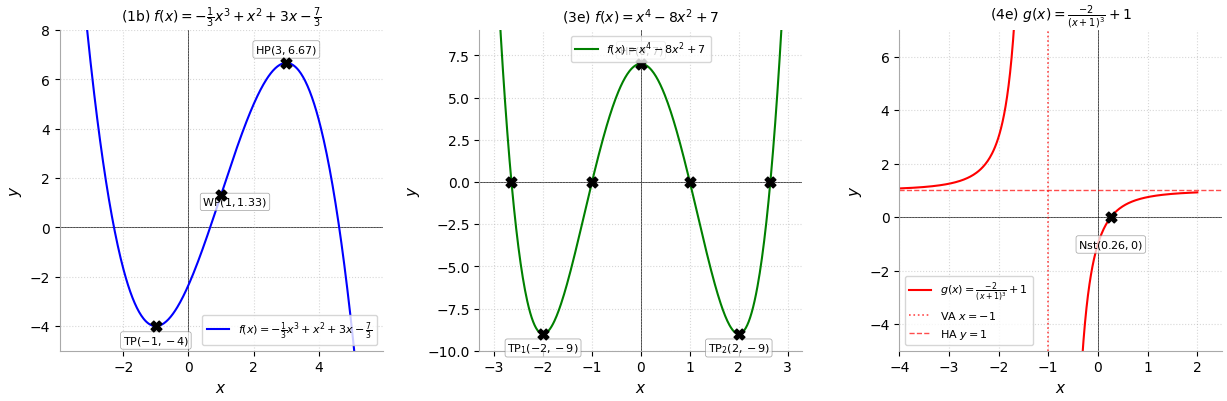
\includegraphics[width=0.8\textwidth]{grafiken/uebergreifend_alle_graphen.png}
% --- Beschreibung der Skizze ---
% Die Skizze sollte zwei Graphen in einem Koordinatensystem zeigen, möglicherweise mit unterschiedlichen y-Achsen oder angepasster Skalierung, um die relevanten Merkmale beider Funktionen darzustellen.
% Graph (a) f(x) = 2sin(x)-x: Start (0,0), HP (pi/3, ca. 0.69), WP (pi, -pi), TP (5pi/3, ca. -6.97), Ende (2pi, -2pi).
% Graph (b) g(x) = x*cos(x): Symmetrisch zum Ursprung. Start (-pi,pi), TP(ca. -0.86, -0.56), Nst/WP (0,0), HP(ca. 0.86, 0.56), Ende (pi,-pi). Nullstellen auch bei +-pi/2.
\captionof{figure}{Graphen der Funktionen $f(x)=2\sin(x)-x$ (im Intervall $[0,2\pi]$) und $g(x)=x\cos(x)$ (im Intervall $[-\pi,\pi]$) (konzeptionell).}
\label{fig:kurvendisk_trig_kombiniert}
\end{center}

\end{loesungsumgebung}


\begin{aufgabenumgebung}{Integrationsregeln im Mix}
Nachdem du nun vielfältige Funktionen und Integrationstechniken kennengelernt hast, soll diese Aufgabe dein Verständnis und deine Fertigkeiten bei der Kombination verschiedener Regeln prüfen.

Berechne die folgenden unbestimmten Integrale. Gib an, welche Methode(n) (z.B. partielle Integration, Substitution, Grundintegrale) du verwendest.
\begin{enumerate}[label=(\alph*)]
    \item $\int x^2 \cos(x) \,dx$
    \item $\int \sin(x) \cdot e^{\cos(x)} \,dx$
    \item $\int e^{2x} \cos(x) \,dx$
    \item \textbf{Für Experten:} $\int \sin(\ln x) \,dx$
    \item \textbf{Flächenberechnung (Herausforderung):} Bestimme den Inhalt der Fläche, die vom Graphen der Funktion $f(x) = e^x \sin(x)$ und der x-Achse im Intervall $[0, \pi]$ eingeschlossen wird. Fertige eine Skizze an. Du benötigst die Stammfunktion aus Aufgabe (c) (oder der früheren Herausforderung). Beachte, dass $\sin(x)$ im Intervall $[0,\pi]$ nicht negativ ist.
\end{enumerate}
Diese Aufgaben erfordern sorgfältiges Anwenden der Regeln und oft auch mehrere Schritte. Viel Erfolg!
\end{aufgabenumgebung}


\begin{loesungsumgebung}[loes:integration-mix-trig-e]{Integrationsregeln im Mix}
Wir berechnen die folgenden unbestimmten Integrale und die gefragte Fläche.

\begin{enumerate}[label=(\alph*)]
    \item $\mathbf{\int x^2 \cos(x) \,dx}$ \\
    Methode: Zweifache partielle Integration.
    \textbf{1. Partielle Integration:} Wähle $f(x)=x^2$ (wird abgeleitet) und $g'(x)=\cos(x)$ (wird integriert).
    $f(x) = x^2 \Rightarrow f'(x) = 2x$.
    $g'(x) = \cos(x) \Rightarrow g(x) = \sin(x)$.
    $$ \int x^2 \cos(x) \,dx = x^2\sin(x) - \int 2x \sin(x) \,dx = x^2\sin(x) - 2 \int x \sin(x) \,dx \quad (*) $$
    \textbf{2. Partielle Integration für $\int x \sin(x) \,dx$:}
    Wähle $f_2(x)=x \Rightarrow f_2'(x)=1$.
    Wähle $g_2'(x)=\sin(x) \Rightarrow g_2(x)=-\cos(x)$.
    $$ \int x \sin(x) \,dx = x(-\cos(x)) - \int 1 \cdot (-\cos(x)) \,dx = -x\cos(x) + \int \cos(x) \,dx = -x\cos(x) + \sin(x) $$
    Setze dies in $(*)$ ein:
    \begin{align*} \int x^2 \cos(x) \,dx &= x^2\sin(x) - 2(-x\cos(x) + \sin(x)) + C \\ &= x^2\sin(x) + 2x\cos(x) - 2\sin(x) + C \\ &= \mathbf{(x^2-2)\sin(x) + 2x\cos(x) + C} \end{align*}

    \item $\mathbf{\int \sin(x) \cdot e^{\cos(x)} \,dx}$ \\
    Methode: Substitution. Der Exponent $\cos(x)$ und seine Ableitung (bis auf Vorzeichen) $\sin(x)$ sind vorhanden.
    Wähle $u = \cos(x)$.
    Dann $\frac{du}{dx} = -\sin(x) \Rightarrow du = -\sin(x) \,dx \Rightarrow \sin(x) \,dx = -du$.
    \begin{align*} \int e^{\cos(x)} \cdot \sin(x) \,dx &= \int e^u (-du) \\ &= -\int e^u \,du \\ &= -e^u + C \end{align*}
    Rücksubstitution $u=\cos(x)$:
    $$ \mathbf{-e^{\cos(x)} + C} $$

    \item $\mathbf{\int e^{2x} \cos(x) \,dx}$ \\
    Methode: Zweifache partielle Integration, dann algebraisches Auflösen nach dem gesuchten Integral $I$.
    Sei $I = \int e^{2x} \cos(x) \,dx$.
    \textbf{1. Partielle Integration:} Wähle $f(x)=\cos(x) \Rightarrow f'(x)=-\sin(x)$. Wähle $g'(x)=e^{2x} \Rightarrow g(x)=\frac{1}{2}e^{2x}$.
    $$ I = \cos(x) \cdot \frac{1}{2}e^{2x} - \int (-\sin(x)) \cdot \frac{1}{2}e^{2x} \,dx = \frac{1}{2}e^{2x}\cos(x) + \frac{1}{2} \int e^{2x}\sin(x) \,dx \quad (1) $$
    \textbf{2. Partielle Integration für $J = \int e^{2x}\sin(x) \,dx$:}
    Wähle $u_2(x)=\sin(x) \Rightarrow u_2'(x)=\cos(x)$. Wähle $v_2'(x)=e^{2x} \Rightarrow v_2(x)=\frac{1}{2}e^{2x}$.
    $$ J = \sin(x) \cdot \frac{1}{2}e^{2x} - \int \cos(x) \cdot \frac{1}{2}e^{2x} \,dx = \frac{1}{2}e^{2x}\sin(x) - \frac{1}{2}I $$
    Setze $J$ in (1) ein:
    $$ I = \frac{1}{2}e^{2x}\cos(x) + \frac{1}{2}\left(\frac{1}{2}e^{2x}\sin(x) - \frac{1}{2}I\right) $$
    $$ I = \frac{1}{2}e^{2x}\cos(x) + \frac{1}{4}e^{2x}\sin(x) - \frac{1}{4}I $$
    Löse nach $I$:
    $I + \frac{1}{4}I = \frac{1}{2}e^{2x}\cos(x) + \frac{1}{4}e^{2x}\sin(x)$
    $\frac{5}{4}I = \frac{e^{2x}}{4}(2\cos(x) + \sin(x))$
    $I = \frac{4}{5} \cdot \frac{e^{2x}}{4}(2\cos(x) + \sin(x)) + C$
    $$ \mathbf{\int e^{2x} \cos(x) \,dx = \frac{1}{5}e^{2x}(2\cos(x) + \sin(x)) + C} $$

    \item \textbf{Für Experten: $\int \sin(\ln x) \,dx$} \\
    Methode: Zuerst Substitution, dann zweifache partielle Integration.
    \textbf{1. Substitution:} Wähle $u = \ln x$. Dann ist $x = e^u$, und $\frac{dx}{du} = e^u \Rightarrow dx = e^u \,du$.
    Das Integral wird zu $\int \sin(u) e^u \,du$.
    \textbf{2. Partielle Integration für $\int e^u \sin(u) \,du$:}
    Dies ist ein bekanntes 'Trick-Integral' (siehe vorherige Aufgaben oder Herleitung unten).
    Sei $K = \int e^u \sin(u) \,du$.
    Wähle $f(u)=\sin u \Rightarrow f'(u)=\cos u$. Wähle $g'(u)=e^u \Rightarrow g(u)=e^u$.
    $K = e^u \sin u - \int e^u \cos u \,du$.
    Für $\int e^u \cos u \,du$: Wähle $f_2(u)=\cos u \Rightarrow f_2'(u)=-\sin u$. Wähle $g_2'(u)=e^u \Rightarrow g_2(u)=e^u$.
    $\int e^u \cos u \,du = e^u \cos u - \int e^u (-\sin u) \,du = e^u \cos u + K$.
    Einsetzen: $K = e^u \sin u - (e^u \cos u + K)$.
    $K = e^u \sin u - e^u \cos u - K \Rightarrow 2K = e^u(\sin u - \cos u) \Rightarrow K = \frac{1}{2}e^u(\sin u - \cos u)$.
    \textbf{3. Rücksubstitution:} $u=\ln x$, $e^u=x$.
    $$ \mathbf{\int \sin(\ln x) \,dx = \frac{1}{2}x(\sin(\ln x) - \cos(\ln x)) + C} $$

    \item \textbf{Flächenberechnung (Herausforderung): $f(x) = e^x \sin(x)$ im Intervall $[0, \pi]$.}
    \begin{itemize}
        \item \textbf{Stammfunktion:} Aus Teil (d) (mit $u$ statt $x$) oder einer früheren Aufgabe wissen wir: $\int e^x \sin(x) \,dx = \frac{1}{2}e^x(\sin x - \cos x) + C$.
        \item \textbf{Vorzeichen von $f(x)$ im Intervall $[0, \pi]$:}
        Für $x \in [0, \pi]$ ist $e^x > 0$.
        Für $x \in [0, \pi]$ ist $\sin(x) \ge 0$.
        Also ist $f(x) = e^x \sin(x) \ge 0$ für $x \in [0, \pi]$.
        Der Flächeninhalt $A$ ist daher $A = \int_0^\pi e^x \sin(x) \,dx$.
        \item \textbf{Berechnung des bestimmten Integrals:}
        \begin{align*} A &= \left[ \frac{1}{2}e^x(\sin x - \cos x) \right]_0^\pi \\ &= \frac{1}{2}e^\pi(\sin\pi - \cos\pi) - \frac{1}{2}e^0(\sin 0 - \cos 0) \\ &= \frac{1}{2}e^\pi(0 - (-1)) - \frac{1}{2}(1)(0 - 1) \\ &= \frac{1}{2}e^\pi(1) - \frac{1}{2}(-1) \\ &= \frac{1}{2}e^\pi + \frac{1}{2} = \mathbf{\frac{1}{2}(e^\pi + 1)} \end{align*}
        Numerisch: $A \approx \frac{1}{2}(23.14069 + 1) \approx \frac{24.14069}{2} \approx 12.070$ Flächeneinheiten.
        \item \textbf{Skizze (textuell):} Der Graph von $f(x)=e^x\sin x$ startet bei $(0,0)$. Da $e^x$ positiv ist und wächst, und $\sin x$ zwischen $0$ und $1$ oszilliert (für $x \in [0,\pi]$), beschreibt die Funktion einen 'Berg' oberhalb der x-Achse, der bei $x=0$ beginnt, bei $x=\pi$ wieder die x-Achse erreicht, und dazwischen eine Amplitude hat, die durch $e^x$ beeinflusst wird (der Hochpunkt liegt vor $x=\pi/2$ wegen des $e^x$ Faktors). Die berechnete Fläche ist der Inhalt dieses ersten positiven 'Berges' der Funktion $e^x \sin x$. Die Abbildung \ref{fig:flaeche_xplus1ehochminusx} im Aufgabentext bezieht sich auf eine andere Funktion.
    \end{itemize}
\end{enumerate}

\end{loesungsumgebung}




\begin{aufgabenumgebung}{Checkliste: Bogenmaß, Einheitskreis und Grundeigenschaften verstehen}
Die Basis der trigonometrischen Funktionen liegt im Einheitskreis und der Verwendung des Bogenmaßes. Überprüfe dein Verständnis:

\begin{enumerate}[label=(\alph*)]
    \item \textbf{Bogenmaß vs. Gradmaß:}
    \begin{itemize}
        \item Erkläre mit eigenen Worten, was das Bogenmaß eines Winkels darstellt. Warum ist $180^\circ = \pi \text{ rad}$?
        \item Warum ist es in der Analysis (insbesondere beim Ableiten) wichtig, Winkel im Bogenmaß anzugeben? (Tipp: Denke an die Einfachheit der Ableitungsformeln.)
    \end{itemize}
    \item \textbf{Sinus und Kosinus am Einheitskreis:}
    \begin{itemize}
        \item Wie hängen die Koordinaten eines Punktes $P(x_P|y_P)$ auf dem Einheitskreis mit $\sin(\alpha)$ und $\cos(\alpha)$ zusammen, wenn $\alpha$ der Winkel zwischen der positiven x-Achse und dem Strahl zum Punkt $P$ ist?
        \item Erkläre mithilfe des Einheitskreises, warum der Wertebereich von $\sin(x)$ und $\cos(x)$ das Intervall $[-1, 1]$ ist.
        \item Leite die Identität $\sin^2(x) + \cos^2(x) = 1$ (Trigonometrischer Pythagoras) aus der Definition am Einheitskreis her.
    \end{itemize}
    \item \textbf{Periodizität und Symmetrie:}
    \begin{itemize}
        \item Was bedeutet es, dass $\sin(x)$ und $\cos(x)$ periodisch mit der Periode $2\pi$ sind? Wie zeigt sich das am Einheitskreis und im Graphen?
        \item Erkläre die Punktsymmetrie von $\sin(x)$ zum Ursprung ($\sin(-x)=-\sin x$) und die Achsensymmetrie von $\cos(x)$ zur y-Achse ($\cos(-x)=\cos x$) anhand des Einheitskreises.
    \end{itemize}
\end{enumerate}
\end{aufgabenumgebung}


\begin{loesungsumgebung}[loes:checkliste-bogenmass-einheitskreis]{Checkliste: Bogenmaß, Einheitskreis und Grundeigenschaften verstehen}

\begin{enumerate}[label=(\alph*)]
    \item \textbf{Bogenmaß vs. Gradmaß:}
    \begin{itemize}
        \item \textbf{Erklärung Bogenmaß und $180^\circ = \pi \text{ rad}$:} \\
        Das \textbf{Bogenmaß} eines Winkels ist definiert als das Verhältnis der Länge des Kreisbogens $s$, den der Winkel aus einem Kreis mit Radius $r$ ausschneidet, zum Radius $r$ dieses Kreises. Die Formel lautet $\alpha_{rad} = \frac{s}{r}$. Das Bogenmaß ist dimensionslos, oft wird die Einheit 'Radiant' (rad) hinzugefügt.
        Am \textbf{Einheitskreis} (Radius $r=1$) entspricht das Bogenmaß eines Winkels direkt der Länge des zugehörigen Kreisbogens ($s=\alpha_{rad}$).
        Ein Winkel von $180^\circ$ beschreibt einen Halbkreis. Der Umfang eines Kreises mit Radius $r$ ist $2\pi r$. Die Länge des Bogens eines Halbkreises ist somit $\frac{1}{2} \cdot 2\pi r = \pi r$. Im Einheitskreis ($r=1$) ist diese Bogenlänge $\pi \cdot 1 = \pi$. Daher entspricht der Winkel $180^\circ$ dem Bogenmaß $\mathbf{\pi}$ Radiant.

        \item \textbf{Wichtigkeit des Bogenmaßes in der Analysis:} \\
        In der Analysis, insbesondere beim Differenzieren und Integrieren trigonometrischer Funktionen, ist die Verwendung des Bogenmaßes unerlässlich. Die einfachen Ableitungsformeln wie $(\sin x)' = \cos x$ und $(\cos x)' = -\sin x$ gelten \textbf{nur}, wenn der Winkel $x$ im Bogenmaß angegeben ist. Würde man das Gradmaß verwenden, träten in diesen Formeln zusätzliche konstante Faktoren ($\frac{\pi}{180}$) auf, was die Rechnungen verkomplizieren würde (z.B. wäre die Ableitung von $\sin(x^\circ)$ gleich $\frac{\pi}{180}\cos(x^\circ)$). Das Bogenmaß ist die 'natürliche' Maßeinheit für Winkel in der höheren Mathematik, da es einen direkten geometrischen Bezug zur Bogenlänge am Einheitskreis hat.
    \end{itemize}

    \item \textbf{Sinus und Kosinus am Einheitskreis:}
    \begin{itemize}
        \item \textbf{Zusammenhang zwischen Koordinaten und $\sin(\alpha), \cos(\alpha)$:} \\
        Betrachtet man einen Punkt $P(x_P|y_P)$ auf dem Einheitskreis (Kreis mit Mittelpunkt im Ursprung und Radius 1), so sind seine Koordinaten direkt durch den Winkel $\alpha$ definiert, der von der positiven x-Achse gegen den Uhrzeigersinn zum Strahl $OP$ (vom Ursprung zum Punkt $P$) gemessen wird:
        Die \textbf{x-Koordinate} des Punktes $P$ ist $\mathbf{x_P = \cos(\alpha)}$.
        Die \textbf{y-Koordinate} des Punktes $P$ ist $\mathbf{y_P = \sin(\alpha)}$.

        \item \textbf{Erklärung des Wertebereichs $[-1, 1]$:} \\
        Da der Einheitskreis den Radius 1 hat und sein Mittelpunkt im Ursprung liegt, können die x-Koordinaten und y-Koordinaten der Punkte auf diesem Kreis nicht kleiner als -1 und nicht größer als 1 sein.
        Da $\cos(\alpha)$ die x-Koordinate und $\sin(\alpha)$ die y-Koordinate eines Punktes auf dem Einheitskreis ist, gilt:
        $-1 \le \cos(\alpha) \le 1$
        $-1 \le \sin(\alpha) \le 1$
        Der Wertebereich von $\sin(x)$ und $\cos(x)$ ist daher jeweils das abgeschlossene Intervall $\mathbf{[-1, 1]}$.

        \item \textbf{Herleitung $\sin^2(x) + \cos^2(x) = 1$ (Trigonometrischer Pythagoras):} \\
        Die Gleichung des Einheitskreises lautet $x_P^2 + y_P^2 = r^2$. Mit $r=1$ ist dies $x_P^2 + y_P^2 = 1$.
        Da $x_P = \cos(x)$ und $y_P = \sin(x)$, können wir diese Definitionen in die Kreisgleichung einsetzen:
        $(\cos x)^2 + (\sin x)^2 = 1$.
        Dies wird üblicherweise als $\mathbf{\sin^2(x) + \cos^2(x) = 1}$ geschrieben und wird als 'Trigonometrischer Pythagoras' bezeichnet, da es direkt aus dem Satz des Pythagoras in dem rechtwinkligen Dreieck resultiert, das durch den Punkt $P$ auf dem Einheitskreis, den Ursprung und die Projektion von $P$ auf die x-Achse gebildet wird (Hypotenuse ist der Radius 1, die Katheten haben die Längen $|\cos x|$ und $|\sin x|$).
    \end{itemize}

    \item \textbf{Periodizität und Symmetrie:}
    \begin{itemize}
        \item \textbf{Bedeutung der Periodizität mit Periode $2\pi$:} \\
        Dass $\sin(x)$ und $\cos(x)$ periodisch mit der Periode $2\pi$ sind, bedeutet, dass sich ihre Funktionswerte alle $2\pi$ wiederholen:
        $\sin(x + 2k\pi) = \sin(x)$ und $\cos(x + 2k\pi) = \cos(x)$ für jede ganze Zahl $k$.
        \textbf{Am Einheitskreis:} Ein Winkel von $2\pi$ Radiant entspricht einer vollen Umdrehung (360°). Addiert man zu einem Winkel $\alpha$ ein Vielfaches von $2\pi$, so landet man wieder am selben Punkt auf dem Einheitskreis. Da $\sin(\alpha)$ und $\cos(\alpha)$ die Koordinaten dieses Punktes sind, bleiben sie unverändert.
        \textbf{Im Graphen:} Die Graphen der Sinus- und Kosinusfunktion zeigen ein sich wiederholendes Muster (eine 'Welle'). Die Länge dieses Musters entlang der x-Achse beträgt $2\pi$.

        \item \textbf{Erklärung der Symmetrien anhand des Einheitskreises:}
        \begin{itemize}
            \item \textbf{Punktsymmetrie von $\sin(x)$ zum Ursprung ($\sin(-x)=-\sin x$):}
            Betrachtet man einen Winkel $x$ und den Winkel $-x$ am Einheitskreis, so liegt der Punkt $P_1(\cos x | \sin x)$ auf dem Einheitskreis. Der Punkt $P_2(\cos(-x) | \sin(-x))$ für den Winkel $-x$ ergibt sich durch Spiegelung von $P_1$ an der x-Achse. Dabei bleibt die x-Koordinate gleich ($\cos(-x)=\cos x$), aber die y-Koordinate kehrt ihr Vorzeichen um ($\sin(-x)=-\sin x$). Da $f(-x)=-f(x)$ für $f(x)=\sin x$, ist Sinus eine ungerade Funktion, und ihr Graph ist punktsymmetrisch zum Ursprung.
            \item \textbf{Achsensymmetrie von $\cos(x)$ zur y-Achse ($\cos(-x)=\cos x$):}
            Wie oben erwähnt, bleibt die x-Koordinate bei Spiegelung des Winkels an der x-Achse gleich: $\cos(-x)=\cos x$. Da $f(-x)=f(x)$ für $f(x)=\cos x$, ist Kosinus eine gerade Funktion, und ihr Graph ist achsensymmetrisch zur y-Achse.
        \end{itemize}
    \end{itemize}
\end{enumerate}

\end{loesungsumgebung}

\begin{aufgabenumgebung}{Checkliste: Transformationen und Analysis trigonometrischer Funktionen}
Die Grundfunktionen $\sin(x)$ und $\cos(x)$ können transformiert und mit den Werkzeugen der Differential- und Integralrechnung analysiert werden.

\begin{enumerate}[label=(\alph*)]
    \item \textbf{Transformierte Sinusfunktion $f(x) = A \sin(B(x-C)) + D$:}
    \begin{itemize}
        \item Wenn du eine Schwingung modellieren möchtest, die doppelt so hoch ausschlägt wie $\sin(x)$ und nur halb so schnell schwingt (also die doppelte Periode hat), wie müsstest du $A$ und $B$ wählen (angenommen $A>0, B>0$)?
        \item Wie verschiebt sich der 'Standard-Startpunkt' (der bei $\sin(x)$ im Ursprung mit positiver Steigung liegt) durch die Parameter $C$ und $D$? Was ist die Gleichung der Mittellage?
    \end{itemize}
    \item \textbf{Ableitungen und ihre Bedeutung:}
    \begin{itemize}
        \item Es gilt $(\sin x)' = \cos x$. Betrachte die Graphen von $\sin x$ und $\cos x$: An welchen Stellen hat $\sin x$ seine Extrempunkte (Hoch-/Tiefpunkte)? Was ist an diesen Stellen der Wert von $\cos x$ (also der Ableitung)? Passt das zur Regel, dass die Ableitung an Extremstellen Null ist?
        \item Umgekehrt: Wo hat $\cos x$ seine Nullstellen? Was für Punkte (bezüglich Steigung) hat $\sin x$ an diesen Stellen?
        \item Warum ist das Vorzeichen bei $(\cos x)' = -\sin x$ negativ? Versuche, dies anhand der Steigung des Kosinusgraphen zu erklären, wenn $\sin x$ positiv ist.
    \end{itemize}
    \item \textbf{Integration und Fläche:}
    \begin{itemize}
        \item Das bestimmte Integral $\int_0^{2\pi} \cos(x) \,dx = 0$. Erkläre dieses Ergebnis geometrisch anhand des Graphen von $\cos(x)$ und dem Konzept der orientierten Fläche.
        \item Wie würdest du vorgehen, um den \textit{gesamten geometrischen Flächeninhalt} zu berechnen, den der Graph von $f(x)=\sin(x)$ mit der x-Achse im Intervall $[0, 2\pi]$ einschließt? (Tipp: Nullstellen und Beträge).
    \end{itemize}
    \item \textbf{Tangensfunktion:}
    \begin{itemize}
        \item Warum ist die Tangensfunktion $\tan(x) = \frac{\sin x}{\cos x}$ nicht für alle $x \in \mathbb{R}$ definiert? Was befindet sich an den Definitionslücken im Graphen?
        \item Die Ableitung von $\tan x$ ist $(\tan x)' = \frac{1}{\cos^2 x}$. Ist diese Ableitung jemals negativ? Was bedeutet das für die Monotonie der Tangensfunktion in ihren Definitionsintervallen?
    \end{itemize}
\end{enumerate}
\end{aufgabenumgebung}


\begin{loesungsumgebung}[loes:checkliste-trig-analysis]{Checkliste: Transformationen und Analysis trigonometrischer Funktionen}

\begin{enumerate}[label=(\alph*)]
    \item \textbf{Transformierte Sinusfunktion $f(x) = A \sin(B(x-C)) + D$:}
    \begin{itemize}
        \item \textbf{Wahl von $A$ und $B$ für veränderte Schwingung:}
        Eine Schwingung, die im Vergleich zu $\sin(x)$ (Amplitude 1, Periode $2\pi$) \textbf{doppelt so hoch ausschlägt}, hat die Amplitude $|A|=2$. Da $A>0$ gefordert ist, ist $\mathbf{A=2}$.
        Eine Schwingung, die \textbf{halb so schnell schwingt}, hat die doppelte Periode, also $P_{neu} = 2 \cdot 2\pi = 4\pi$. Die Periode ist gegeben durch $P = \frac{2\pi}{|B|}$. Mit $B>0$ und $P_{neu}=4\pi$ folgt:
        $4\pi = \frac{2\pi}{B} \Rightarrow B = \frac{2\pi}{4\pi} = \mathbf{\frac{1}{2}}$.

        \item \textbf{Verschiebung des 'Standard-Startpunkts' und Mittellage:}
        Der 'Standard-Startpunkt' von $\sin(x)$ ist der Ursprung $(0|0)$, wo die Funktion mit positiver Steigung ihre Mittellinie (die x-Achse, $y=0$) kreuzt.
        \begin{itemize}
            \item Der Parameter $\mathbf{C}$ bewirkt eine horizontale Verschiebung. In $A \sin(B(x-C))+D$ ist der Punkt, an dem das Argument der Sinusfunktion ($B(x-C)$) Null ist, bei $x-C=0 \Rightarrow x=C$. Dieser Punkt $(C,D)$ entspricht dem verschobenen Ursprung der Grundsinuskurve (Startpunkt der Periode, Anstieg durch die Mittellinie, wenn $A>0$). Eine Verschiebung um $C$ nach rechts (wenn $C>0$) oder links (wenn $C<0$).
            \item Der Parameter $\mathbf{D}$ bewirkt eine vertikale Verschiebung um $D$ Einheiten. Die Mittellinie der Schwingung wird von $y=0$ auf $\mathbf{y=D}$ verschoben.
        \end{itemize}
    \end{itemize}

    \item \textbf{Ableitungen und ihre Bedeutung:}
    \begin{itemize}
        \item \textbf{$(\sin x)' = \cos x$. Extrema von $\sin x$ vs. Wert von $\cos x$:}
        Die Funktion $\sin x$ hat ihre Extrempunkte (Hoch- oder Tiefpunkte) an den Stellen $x = \frac{\pi}{2} + k\pi$ (für $k \in \mathbb{Z}$), also bei $\frac{\pi}{2}, \frac{3\pi}{2}, \frac{5\pi}{2}, \dots$.
        An diesen Stellen ist die Tangente an den Graphen von $\sin x$ horizontal, d.h., die Steigung ist Null.
        Der Wert von $\cos x$ (der Ableitung von $\sin x$) an diesen Stellen ist:
        $\cos(\frac{\pi}{2}) = 0$, $\cos(\frac{3\pi}{2}) = 0$, $\cos(\frac{5\pi}{2}) = 0$, usw.
        Dies passt exakt zur Regel, dass die Ableitung einer Funktion an ihren Extremstellen Null ist (notwendige Bedingung).

        \item \textbf{Nullstellen von $\cos x$ und Steigung von $\sin x$ an diesen Stellen:}
        Die Funktion $\cos x$ hat ihre Nullstellen an den Stellen $x = \frac{\pi}{2} + k\pi$ (für $k \in \mathbb{Z}$).
        Dies sind genau die Stellen, an denen $\sin x$ seine Extremwerte ($1$ oder $-1$) annimmt. An diesen Extremstellen hat der Graph von $\sin x$ eine horizontale Tangente, was bedeutet, dass seine Steigung Null ist. Die Steigung von $\sin x$ wird durch $(\sin x)' = \cos x$ beschrieben, und an den Nullstellen von $\cos x$ ist die Steigung von $\sin x$ folgerichtig Null.

        \item \textbf{Warum ist das Vorzeichen bei $(\cos x)' = -\sin x$ negativ?}
        Betrachten wir den Graphen der Kosinusfunktion. Zum Beispiel im Intervall $(0, \pi)$:
        \begin{itemize}
            \item Für $x \in (0, \pi)$ ist $\sin x > 0$.
            \item Im gleichen Intervall $(0, \pi)$ fällt der Graph von $\cos x$ stetig (von $\cos 0 = 1$ zu $\cos \pi = -1$). Die Steigung des Kosinusgraphen ist also in diesem gesamten Intervall negativ.
        \end{itemize}
        Da $\sin x$ im Intervall $(0, \pi)$ positiv ist, muss die Ableitung von $\cos x$ ein negatives Vorzeichen enthalten ($-\sin x$), um die beobachtete negative Steigung des Kosinusgraphen korrekt wiederzugeben. Wenn $\sin x$ positiv ist, bedeutet $-\sin x$, dass die Steigung von $\cos x$ negativ ist, was dem fallenden Verlauf von $\cos x$ in diesem Bereich entspricht.
    \end{itemize}

    \item \textbf{Integration und Fläche:}
    \begin{itemize}
        \item \textbf{Geometrische Erklärung für $\int_0^{2\pi} \cos(x) \,dx = 0$:}
        Das bestimmte Integral $\int_0^{2\pi} \cos(x) \,dx$ repräsentiert die orientierte Fläche zwischen dem Graphen von $\cos(x)$ und der x-Achse im Intervall $[0, 2\pi]$.
        \begin{itemize}
            \item Im Intervall $[0, \frac{\pi}{2}]$ ist $\cos(x) \ge 0$, die Fläche $A_1 = \int_0^{\pi/2} \cos x \,dx = [\sin x]_0^{\pi/2} = 1$.
            \item Im Intervall $[\frac{\pi}{2}, \frac{3\pi}{2}]$ ist $\cos(x) \le 0$. Die Fläche $A_2 = \int_{\pi/2}^{3\pi/2} \cos x \,dx = [\sin x]_{\pi/2}^{3\pi/2} = \sin(3\pi/2) - \sin(\pi/2) = -1 - 1 = -2$.
            \item Im Intervall $[\frac{3\pi}{2}, 2\pi]$ ist $\cos(x) \ge 0$. Die Fläche $A_3 = \int_{3\pi/2}^{2\pi} \cos x \,dx = [\sin x]_{3\pi/2}^{2\pi} = \sin(2\pi) - \sin(3\pi/2) = 0 - (-1) = 1$.
        \end{itemize}
        Die Gesamtbilanz der orientierten Flächen ist $A_1 + A_2 + A_3 = 1 + (-2) + 1 = 0$.
        Die positiven Flächenstücke (oberhalb der x-Achse) und das negative Flächenstück (unterhalb der x-Achse) heben sich exakt auf.

        \item \textbf{Berechnung des gesamten geometrischen Flächeninhalts von $f(x)=\sin(x)$ mit der x-Achse im Intervall $[0, 2\pi]$:}
        Die Nullstellen von $\sin(x)$ im Intervall $[0, 2\pi]$ sind $x=0, x=\pi, x=2\pi$.
        \begin{itemize}
            \item Im Intervall $[0, \pi]$ ist $\sin(x) \ge 0$. Die Fläche ist $A_1 = \int_0^\pi \sin(x) \,dx = [-\cos x]_0^\pi = (-\cos\pi) - (-\cos 0) = (-(-1)) - (-1) = 1+1=2$.
            \item Im Intervall $[\pi, 2\pi]$ ist $\sin(x) \le 0$. Die Fläche ist $A_2 = \int_\pi^{2\pi} |\sin(x)| \,dx = -\int_\pi^{2\pi} \sin(x) \,dx$.
            $-\int_\pi^{2\pi} \sin(x) \,dx = -[-\cos x]_\pi^{2\pi} = -((-\cos 2\pi) - (-\cos \pi)) = -((-1) - (-(-1))) = -(-1-1) = -(-2) = 2$.
        \end{itemize}
        Der gesamte geometrische Flächeninhalt ist die Summe der Beträge der Flächen über den Teilintervallen, in denen die Funktion nicht das Vorzeichen wechselt: $A_{geom} = A_1 + A_2 = 2+2 = \mathbf{4}$.
    \end{itemize}

    \item \textbf{Tangensfunktion:}
    \begin{itemize}
        \item \textbf{Warum ist $\tan(x) = \frac{\sin x}{\cos x}$ nicht für alle $x \in \mathbb{R}$ definiert? Was befindet sich an den Definitionslücken?} \\
        Die Tangensfunktion ist als $\tan(x) = \frac{\sin x}{\cos x}$ definiert. Sie ist nicht definiert, wenn der Nenner $\cos x$ gleich Null ist.
        Dies ist der Fall für $x = \frac{\pi}{2} + k\pi$, wobei $k$ eine beliebige ganze Zahl ist (z.B. $\pm\frac{\pi}{2}, \pm\frac{3\pi}{2}, \dots$).
        An diesen Definitionslücken hat der Graph der Tangensfunktion \textbf{senkrechte Asymptoten} (Polstellen). Wenn sich $x$ diesen Werten nähert, gehen die Funktionswerte $\tan(x)$ gegen $+\infty$ oder $-\infty$.

        \item \textbf{Ableitung $(\tan x)' = \frac{1}{\cos^2 x}$. Ist sie jemals negativ? Bedeutung für Monotonie?} \\
        Die Ableitung der Tangensfunktion ist $(\tan x)' = \frac{1}{\cos^2 x}$.
        \begin{itemize}
            \item Der Term $\cos^2 x$ ist immer größer oder gleich Null. In den Definitionsintervallen von $\tan x$ ist $\cos x \neq 0$, also ist $\cos^2 x > 0$.
            \item Der Zähler ist $1$ (positiv).
        \end{itemize}
        Daher ist $\frac{1}{\cos^2 x}$ immer positiv für alle $x$, für die $\tan x$ definiert ist. Die Ableitung ist also \textbf{niemals negativ}.
        \textit{Bedeutung für die Monotonie:} Da die Ableitung $(\tan x)'$ in jedem Definitionsintervall von $\tan x$ strikt positiv ist, ist die Tangensfunktion in jedem dieser Intervalle \textbf{streng monoton steigend}.
    \end{itemize}
\end{enumerate}

\end{loesungsumgebung}